%\documentclass[iop, usenatbib]{emulateapj}
%\documentclass[iop, usenatbib]{aa}
\documentclass{aa}
%\documentclass[referee]{aa}

%\usepackage[utf8]{inputenc}
\usepackage[varg]{txfonts}

%\usepackage[T1]{fontenc} 
%\usepackage[utf8]{inputenc}

%\usepackage[T1]{fontenc}
%\usepackage[utf8]{inputenc}
%\usepackage{newunicodechar}

\usepackage{amsmath}
\usepackage{amssymb}
\usepackage{epsfig}
\usepackage{graphics}
\usepackage{color}
\usepackage{natbib}
\usepackage{caption}
%\usepackage{siunitx}
%\usepackage{xifthen}

\bibpunct{(}{)}{;}{a}{}{,} % to follow the A&A style

%Debug addition for collaborators
%\usepackage[switch, displaymath, modulo]{lineno}
%\linenumbers
%%\renewcommand\linenumberfont{\color{red}\normalfont\tiny\sffamily}
%\renewcommand\linenumberfont{\normalfont\tiny\sffamily}
%\usepackage{natbib,twoopt}




%Collides with emulateapj
%%%%%%%%%
%\usepackage{siunitx}
% Units
%\DeclareSIUnit{\erg}{erg}
%%%%%%%%%

\DeclareUnicodeCharacter{00A0}{ }

%Commands
\newcommand{\be}{\begin{equation}}
\newcommand{\ee}{\end{equation}}
%\newcommand{\bea}{\begin{eqnarray}}
%\newcommand{\eea}{\end{eqnarray}}
%\newcommand{\bea}{\begin{align}\begin{split}}
%\newcommand{\eea}{\end{split}\end{align}}
\newcommand{\ud}{\text{d}}

%normal 3-vectors
%\renewcommand{\vec}[1]{\ensuremath{\mathbf{#1}}}
%\renewcommand{\vec}[1]{\ensuremath{\boldsymbol{#1}}​}
\renewcommand{\vec}[1]{\ensuremath{\boldsymbol{#1}}}

%four-vectors
\makeatletter
\def\fvec#1{\underline{\sbox\tw@{$#1$}\dp\tw@\z@\box\tw@}}
\makeatother

%highlight color
\newcommand{\red}[1]{\textcolor{red}{#1}}
\newcommand{\pp}[1]{\textcolor{magenta}{\protect{#1}}}
\usepackage[normalem]{ulem}
\newcommand{\ppst}[1]{\textcolor{magenta}{\protect{\sout{#1}}}}


\newcommand{\refe}[1]{\textcolor{green}{{#1}}}
\newcommand{\refedel}[1]{\textcolor{red}{\sout{#1}}}


%general shortcuts
\newcommand{\pd}{\ensuremath{\partial}} %partial derivative
\newcommand{\rg}{\ensuremath{r_{\mathrm{g}}}}
\newcommand{\Req}{\ensuremath{R_{\mathrm{e}}}}
\newcommand{\sch}{Schwarzschild }
\newcommand{\Ca}{\ensuremath{\mathcal{C}}}

\newcommand{\rb}{\ensuremath{\bar{r}}}
\newcommand{\ub}{\ensuremath{\bar{u}}}
\newcommand{\wb}{\ensuremath{\bar{\omega}}}
\newcommand{\Ob}{\ensuremath{\hat{\Omega}}}
\newcommand{\nub}{\ensuremath{\bar{\nu}}}
\newcommand{\zetab}{\ensuremath{\bar{\zeta}}}
\newcommand{\Bb}{\ensuremath{\bar{B}}}
\newcommand{\mub}{\ensuremath{\bar{\mu}}}

\newcommand{\vw}{\ensuremath{v_{\omega}}}
\newcommand{\vz}{\ensuremath{v_{\mathrm{z}}}}

\newcommand{\Msun}{\ensuremath{M_{\odot}}}
\newcommand{\lgamma}{\gamma_{\text{L}}}
\newcommand{\qinv}{\ensuremath{q_{\mathrm{inv}}}}

\renewcommand{\deg}{\ensuremath{^{\circ}}}

%%%%%%%%%%%%%%%%%%%%%%

\begin{document}
\title{Radiation from rapidly rotating oblate neutron stars}

\author{J.\,N\"attil\"a\inst{1,2} \and P. Pihajoki\inst{3} }

\institute{Tuorla Observatory, Department of Physics and Astronomy, University of Turku, V\"ais\"al\"antie 20, FI-21500 Piikki\"o, Finland \email{joonas.a.nattila@utu.fi}
  \and Nordita, KTH Royal Institute of Technology and Stockholm University, Roslagstullsbacken 23, SE-10691 Stockholm, Sweden
  \and University of Helsinki, Department of Physics, Gustaf H\"allstr\"omin katu 2a, 00560 Helsinki, Finland
}

\date{Received XXX / Accepted XXX}



\abstract{
A theoretical framework for emission originating from rapidly rotating oblate compact objects is described in detail.
By using a Hamilton-Jacobi formalism, we show how the special relativistic rotational effects such as aberration of angles, Doppler boosting, and time dilatation naturally emerge from the general relativistic treatment of rotating compact objects.
We use the Butterworth--Ipser metric expanded up to the second order in rotation and hence include effects of light bending, frame-dragging, and quadrupole deviations to our geodesic calculations.
We also give detailed descriptions of the numerical algorithms used and provide an open source implementation of the numerical framework called \textsc{bender}.
As an application, we study spectral line profiles (i.e., smearing kernels) from rapidly rotating oblate neutron stars. 
We find that in this metric description the second order quadrupole effects are not strong enough to produce narrow observable features in the spectral energy distribution for almost any physically realistic parameter combination, and hence, actually detecting them is unlikely.
The Full Width at Tenth Maximum and Full Width at Half Maximum of the rotation smearing kernels are also reported for all \refedel{of the possible} viewing angles.
These can be then used to quantitatively estimate the effects of rotational smearing on the observed spectra.
We also calculate accurate pulse profiles and observer skymaps of emission from hot spots on rapidly rotating accreting millisecond pulsars.
These allow us to quantify the strength of the pulse fractions one expects to observe from typical fast spinning millisecond pulsars.
}

\keywords{gravitation - methods: numerical --- radiative transfer --- stars: neutron}

\titlerunning{Radiation from rapidly rotating NSs}
\maketitle


\section{Introduction}
Accurate modeling of the emission from and around compact objects is a complicated combination of radiative processes and relativity.
Not only is the object curving the spacetime around it, and hence affecting the trajectory of photons, but it can also affect the apparent observed radiation as the emitting surface can move with relativistic velocities.
Already existing convenient and modern frameworks for the emission around rotating (typically Kerr) black holes include \textsc{geokerr} \citep{dexter2009}, \textsc{gyoto} \citep{Vincent11}, \textsc{Gray} \citep{CPO13}, \textsc{pandurata} \citep{SK13}, \textsc{astroray} \citep{SM13}, \textsc{heroic} \citep{NZP16}, \textsc{odyssey} \citep{PYY16}, and \textsc{grtrans} \citep{dexter2016} to name a few.
Here we instead focus on the emission from rotating neutron stars, for which the Kerr metric is not a good approximation if the star is rotating rapidly.
By introducing \textsc{bender},%
\footnote{ \url{ http://github.com/natj/bender} } 
we aim to provide a similar publicly available platform for ray tracing problems focused on spinning compact objects.

%\refedel{Compared to black holes, a further complication with neutron stars is that the radiation originates not only from the vicinity of the object but also from the surface of the star itself, which is rapidly rotating.}
%\refedel{This introduces additional complications to the radiative transfer problem: }
%\refedel{We have static general relativistic effects such as bending of photon trajectories similar to black hole calculations, but, in addition, rotational effects such as Doppler boosting and aberration of the observed angles, too.}
%\refe{
%Compared to black holes, a further complication with neutron stars is that the spacetime is not bent by point-like source but by a rotating fluid.
%This introduces additional complications to the ray-tracing problem because in this case the spacetime will not be spherically symmetric.
%}
%\refedel{Combining these effects is a challenging task both theoretically and numerically.}
\refe{Following the path of photons in a spacetime of a rotating neutron star is a challenging task both theoretically and numerically.}
Current and future observations, on the other hand, demand highly accurate models.
For example, computing accurate pulse profiles of hot spots on spinning neutron stars has been recently intensively investigated, motivated by many upcoming or planned new spaceborne X-ray observatories like ESA's \textit{XIPE} \citep{XIPE}, CNSA's \textit{eXTP} \citep{eXTP}, as well as the already deployed ISRO's \textit{Astrosat} \citep{Astrosat} \refe{and NASA's \textit{NICER} \citep{NICER}.}
The expectation is that with accurate pulse profile observations we may be able to better constrain the unknown neutron star equation of state (EoS), using the information encoded in the radiation \citep[see e.g.,][]{LMB13}.

Previous studies of emission from neutron stars (hereafter NSs) are mainly formulated in a way that use a non-rotating curved spacetime metric for bending of the photon paths, with special relativistic corrections to the rotational effects added separately\refedel{, in an ad-hoc manner} (see e.g.,\refe{ \citealt{PFC83,P95, ML98, WM01, PG03, PB06, Lamb09a, Lamb09b, LMB13, ML15}, but also \citealt{BR01} for a general relativistic treatment). } 
Spacetimes in these studies were also typically described by the spherically symmetric \sch metric.

As it has turned out, fast rotation can, however, be a serious complication when considering the observed emission.
First of all, due to a finite pressure supporting the rotating star, the star is squeezed into an oblate spheroid, with the oblateness increasing with increasing rate of rotation \citep{CST94, MS99, MLC07, BBP13, aGM14}.
This bulge in the equator will then distort the gravitational field outside the star.
In Newtonian theory, the next order correction to a non-spherical object (with azimuthal rotational symmetry and reflection symmetry along the equatorial plane) is defined by the quadrupole moment (see e.g., \citealt{LP99}; but also \citealt{PA12}).
%\citep[see e.g.,][]{LP99}.
Introduction of rapid rotation will then not only \refedel{break the spherical symmetry of the object} \refe{make the star oblate} but will also \refe{make the exterior spacetime latitude dependent.}
Pioneering work in computing pulse profiles of such objects were made by \citet{CL05} and \citet{CML07}.
Recently, a general ray tracing formulation in Hartle-Thorne metric-variant was given in \citet{PJ12} and \citet{BPO12}. 
This formulation was used to compute pulse profiles in \citet{PO14}.
Here we seek to provide a similar, but open and publicly available code for solving similar types of problems.
Moreover, we will focus on building a connection between the previous special relativistic formulations where different rotational effects are added separately by hand, and the full rotating general relativistic formulations where all of these effects naturally emerge from the theory.


Main focus of our framework is on the X-ray emission from accreting millisecond pulsars (AMPs) \citep{WvdK98, PW12} and nuclear-powered millisecond pulsars \citep{Watts12}.
We stress, however, that the whole framework presented in this paper is general enough to be applied to any problem of radiation originating from the vicinity of rotating compact objects. 
The radiation from AMPs emerges from hot spots on the surface of a rapidly rotating neutron star. The spots are heated by the infalling accreted material, which is being channeled to the magnetic poles by the neutron star's magnetic field.
The magnetic axis does not need to coincide with the rotational axis of the star and hence pulsations can be observed from the spots that are rotating around the star.
In the case of nuclear-powered millisecond pulsars, quasi-coherent oscillations are observed during a thermonuclear type I X-ray burst.
The mechanism producing the pulses is, however, very similar to the case of AMPs, as an asymmetric bright patch in the burning surface layer is the origin of the observed pulsation.
Accretion can also spin up these objects into extreme rotational velocities: spin frequencies up to 620 Hz have been verified (4U 1608$-$52; \citealt{MC02}) whereas even a typical source has a spin around $400-500$ Hz \citep{Watts12, PTR14}
Hence, if accurate emission is to be studied from these sources, one has to take the oblate shape and (in some cases) the second-order corrections to the spacetime into account.


The paper is structured as follows.
In Section~\ref{sect:theory} we introduce the framework of formulae and the theoretical background needed to compute the emission.
We also describe the numerical methods used to solve the system of equations and present the publicly available code \textsc{bender},%
which implements this framework.
Next, in Section~\ref{sect:appl} we apply the code to various physical problems. \refedel{, mostly related to AMPs.}
We compare our computations with results in literature, when possible, to verify our calculations.
Finally, in Section~\ref{sect:summary} we summarize our work.


%________________________________________________________________


\section{Theory}\label{sect:theory}
\subsection{Space-time metric}\label{sect:spacetime}

\begin{table*}[ht!]\label{tab:coeffs}
%\renewcommand{\arraystretch}{1.4}
\begin{center}
    \caption{Series expansion terms of the metric coefficients up to $\Ob^2$.}
%\begin{small}
\begin{tabular}{l c c c c}
  \hline
  \noalign{\vskip 0.5ex}
              &  $\Ob = 0$  &  $\Ob^1$   & $\Ob^2$  &  error  \\
  \hline
  \noalign{\vskip 2ex}
  $\nub$       &  $\displaystyle \log\left[ 1-\frac{\ub}{2}\right] - \log\left[ 1+\frac{\ub}{2} \right]$ & --- & $\displaystyle +\left(\frac{\beta}{3}-qP_2(\cos\theta) \right)\ub^3 $ & $+\mathcal{O}\left(\Ob^2 \times \ub^4 \right)$ \\[3ex]
  $\Bb$         &  $\displaystyle \left( 1-\frac{\ub}{2} \right) \left(1+\frac{\ub}{2} \right)$ & --- & $\displaystyle+\beta \ub^2$ & $+\mathcal{O}(\Ob^4) \times \mathcal{O}(\ub^4)$ \\[3ex]
  $\zetab$     &  $\displaystyle \log\left[ \left( 1-\frac{\ub}{2} \right) \left(1+\frac{\ub}{2} \right) \right]$ & --- & $\displaystyle +\beta \left( \frac{3}{4}P_2(\cos{\theta}) - \frac{1}{3} \right) \ub^2$ & $+\mathcal{O}(\Ob^2) \times \mathcal{O}(\ub^4)$ \\[3ex]
%  $\wb$       & --- &  $\displaystyle \frac{2G\mathcal{J}}{c^2\rb^3}$ & $\displaystyle -\frac{3}{2}\ub + \mathcal{O}(\ub^2)$ & $+\mathcal{O}(\Ob^3)$ \\[2ex]
  $\wb$       & --- &  $\displaystyle \wb_1 \ub^3 $ & $\displaystyle -3\wb_1 \ub^4 $ & $+ \mathcal{O}(\Ob^3) + \wb_1 \ub^3 \times \mathcal{O}(\ub^2)$ \\[2ex]
  \hline
\end{tabular}
\begin{center}{ 
    Note:
    The angular velocity term of the local inertial frame is simplified by the notation $\wb_1 \equiv 2 j/M$.
}
\end{center}
%\end{small}
\end{center}
\end{table*}

In our following derivations we will use geometric units where $G=c=1$, for gravitational constant $G$, and speed of light $c$.
We also assume metric signature of $(-,+,+,+)$ following the \citet{MTW73} sign convention.
Additionally, when dealing with actual numerical calculations in the code, we set $G M/c^2 = 1$, hence describing lengths in units of \refedel{\sch}\refe{gravitational} radius, where $M$ is the mass of the compact object.


\refedel{The spacetime metric around a static non-rotating spherically symmetric object is given by the well known \sch solution}
\refe{ The exterior spacetime of a static, non-rotating, spherically symmetric mass is described by the well-known Schwarzschild metric}
\be
ds^2  = -(1-u) dt^2 + (1-u)^{-1}dr^2+r^2(d\theta^2+\sin^2\theta d\phi^2),
\ee
\refe{where $r$ is the radial coordinate defined so that the area of a sphere at coordinate time $t$ is $4\pi r^2$, and we set $u \equiv 2M/r$.}
%where $u = 2M/r$ is the dimensionless compactness \refe{parameter} and $r$ is the radial coordinate, defined so that 
%\refedel{an area of a sphere in this coordinate system is the usual $4\pi r^2$ at some fixed time.}

This metric is equivalent to an alternative solution known as isotropic \sch metric \citep[see e.g.][]{MTW73}
\be
\label{eq:ISch}
ds^2 = -\left( \frac{1-\frac{\ub}{2}}{1+\frac{\ub}{2}} \right)^2 dt^2 + \left( 1+\frac{\ub}{2} \right)^4(d\rb^2 + \rb^2(d\theta^2+\sin^2\theta d\phi^2)),
\ee
%where $\rb$ and $\ub=M/\rb$ are the so-called isotropic radial
%coordinate and the corresponding isotropic compactness \refe{parameter},
%respectively. 
\refe{where $\rb$ is the so-called isotropic radial coordinate and we set $\ub \equiv M/\rb$.}
This kind of isotropic metric has the useful feature that surfaces of constant time are conformally flat, and hence the angles are represented without distortion.
This, however, also means that angular isotropic coordinates do not faithfully represent the distances within the spheres nor does the radial coordinate correspond directly to the radial distance.
From here on, we mark all variables related to the isotropic radial coordinate with a bar on top.

Let us consider a rotating compact object.
\refedel{In addition to the dimensionless compactness \refe{parameter} $u(r)$ (or $\ub(\rb)$),} To describe our system we need a dimensionless angular velocity
\be
\Ob = \Omega \left( \frac{\Req^3}{M} \right)^{1/2},
\ee
where $\Omega$ is the angular velocity of a sphere with an equatorial radius $\Req$ and a mass $M$ scaled with the Newtonian mass shedding (Kepler) limit $(M/\Req^3)^{1/2}$ \citep[see][p.29]{rcs}.  
Here $\Req$ is described using the usual \sch radial coordinate and corresponds to the equatorial radius of the star for which $2\pi\Req$ gives the proper length of the circumference \refe{in the rotational equator as measured in the local static frame.}
The asymptotically flat metric near a stationary axisymmetric rotating object in isotropic form is \citep{BW71} 
\begin{align}\begin{split} \label{eq:BWmetric}
ds^2 & = -e^{2\nub} dt^2 +
     \rb^2 \sin^2\theta \Bb^2 e^{-2\nub}(d\phi - \wb dt)^2 + \\
     & e^{2(\zetab-\nub)}(d\rb^2 + \rb^2d\theta^2),
\end{split}\end{align}
%\eea
where $\wb$ is the angular velocity of the local inertial frame and the functions $\nub$, $\Bb$ and $\zetab$ in the metric coefficients can be expanded in the powers of $\Ob$ and $\ub$ \citep{BI76}.
Here $e^{-\nub}$ is the time dilation factor relating the proper time of the local observer to the time at infinity.
Physical interpretation of $\Bb$ follows from the fact that the proper circumference of a circle around the axis of symmetry is $2\pi(e^{-\nub} \Bb \rb \sin\theta)$.
Similarly, the interpretation of $\zetab$ follows from the fact that $e^{\zetab - \nub}$ acts as a conformal (angle preserving) factor of the spacetime. %determining the orthogonality of the 2-surfaces.
Note also how the time and space coordinates are connected in the isotropic metric via the $\nub$-term that also enters both the radial and angular terms.
The zeroth order terms ($\Ob = 0$) of the series expansions are the familiar \sch metric coefficients \refe{expressed in isotropic coordinates} (see Table 1).
%\be
%e^{\nu_0} = (1-\ub/2)/(1+\ub/2),
%\ee
%\be 
%\Bb_0 = (1-\ub/2)(1+\ub/2)
%\ee
%and
%\be
%\zetab_0 = \log \Bb_0.
%\ee

The first order expansion in rotation ($\Ob^1$) is \refedel{formally}\refe{qualitatively} related to Kerr metric.
In this case we introduce an angular velocity term of the local inertial frame $\wb$ that accounts for the frame-dragging effects. 
\refedel{Up to \refe{second} order,} 
\refe{It} can be defined as
\be\label{eq:wbar}
\wb = \frac{2 j}{M} (\ub^3 - 3\ub^4),
\ee
where the dimensionless quantity $j=\mathcal{J}/M^2$ and $\mathcal{J} = I \Omega$ is the star's angular momentum with moment of inertia $I(M,\Omega)$.

The second order expansion ($\Ob^2$) corresponds to a similar approximation as the Hartle-Thorne slow-rotation spacetime \citep{HT68}, which introduces \refe{two} quadrupole moments into the metric.  
These second order multipole moments can be defined via the dimensionless quantities $q$ and $\beta$, the dimensionless moments of energy density and pressure, respectively.
\refe{These are, however, dependent on the selection of a coordinate system.}
The coordinate invariant quadrupole moment\refedel{, on the other hand,} is a combination of these two \refedel{factors}\refe{quantities} and is given in \citet{PA12} \refe{(see eq. (11) therein; see also \citealt{aGM14} and eq. (18))} as
\be
\qinv =  q + \frac{4}{3} \beta.
\ee
\refe{This detail should be taken into account when comparing the strength of the quadrupole deviations between different metric descriptions.}


\citet{YY13} showed that when the NS mass, radius, and spin are known, the star's structure (and hence the surrounding metric) is almost fully characterized by these three quantities only. %\refe{when considering currently viable EoSs.}
In other words, irrespective of the unknown microphysics of the underlying matter, the NS parameters \refe{(such as moment of inertia and coordinate-invariant quadrupole moment)} are \refe{connected} by what are called (approximative) universal relations.
\citet{BBP13} defined empirical relations for these parameters in the Hartle-Thorne metric based on their computations of rotating NSs with various different equations of state.
Later on, \citet{aGM14} refined these relations for the metric representation \eqref{eq:BWmetric} by \citet{BI76}.
In practice, we can then parameterize the previously presented quantities with great accuracy by using only the dimensionless angular velocity $\Ob$ and the compactness \refe{parameter} $x$.
%\be
%x = \frac{M}{\Req}.
%\ee
Note that both of these parameters are defined \refe{in terms of} the equatorial circumferential radius $\Req$ defined in the usual \sch coordinate system.
To the lowest order, these parameterizations are \citep{aGM14}
\be\label{eq:quad}
q = -0.11 \frac{\Ob^2}{x^2},
\ee
\be\label{eq:beta}
\beta = 0.4454 \Ob^2 x,
\ee
and
\be\label{eq:I}
I = \sqrt{x} (1.136 - 2.53 x + 5.6 x^2) M \Req^2.
\ee
Note also that both $q$ and $\beta$ are $\mathcal{O}(\Ob^2)$, \refe{whereas} $j$ is $\mathcal{O}(\Ob)$.
    
It is possible to transform between the \refe{\sch coordinate radius} $r$ and the isotropic $\rb$ coordinates using the relation \citep{FIP86}
\be\label{eq:rb2r}
r = \Bb e^{-\nub} \rb.
\ee

\refe{The relation between the differentials of the two radial coordinates turns out to be}
\be\label{eq:drb2dr}
dr = e^{\zetab} d\rb
\ee
which can be computed using the series representation of \cite{BI76}.

Since the series expansions of the metric coefficients \refe{are expressed in terms of} the isotropic radial coordinate $\rb$, we will favor this \refe{notation} in our derivation.  
However, in some cases we will simplify the equations into a more intuitive form by using the \refe{\sch radial} $r$ coordinate.


\subsection{Oblate shape of the neutron star}\label{sect:oblate}

\begin{figure}
\centering
\includegraphics[width=9cm]{figs/fig1.pdf}
\caption{\label{fig:geom}
Geometry of the system. Here we show the underlying spherical coordinate system with $\phi$ and $\theta$ coordinates along with the Cartesian $(x,y,z)$ coordinate \refe{system}.
In addition, the observer's $\hat{x}-\hat{y}$ image plane is shown as viewed from an inclination angle $i$.
Star is taken to rotate rapidly around the $y$ axis which leads to an oblate (squeezed) shape for the emitting surface, and, hence, the radial vector $\vec{r}$ and the surface normal $\vec{n}$ start to differ from each other.
}
\end{figure}

Due to the rotation and finite pressure supporting the NS, it is not a perfect sphere when it is rotating.  
It, however, retains axisymmetry, and can be approximated with an oblate spheroid.  
Similarly to \refe{the Eqs. \eqref{eq:quad}-\eqref{eq:I},} \citet{aGM14} \refedel{derived}\refe{constructed} an approximate \refe{formulation} for the shape of \refe{the surface of} a rotating neutron star. 
\refe{It is given by} expressing the radius as a function of colatitude $\theta$, as 
\begin{align}\begin{split}\label{eq:radf}
    R(\theta) &= \Req \left( 1 - \frac{\Req - R_{\mathrm{p}}}{\Req} \cos^2\theta \right) \\
              &= \Req [1-\Ob^2 (0.788 - 1.03x) \cos^2 \theta],
\end{split}\end{align}
\refe{where $R(\pi/2) = \Req$ is the radius of the star in its rotational equator and $R_{\mathrm{p}}$ is its radius as measured along the rotation axis.}

Elemental surface area for a spheroid is given as (using the \refe{usual \sch} coordinates)
\be
dS(\theta) = R^2(\theta) \sin\theta \sqrt{1 + f(\theta)^2}d\theta d\phi,
\ee
where
\be
f(\theta) = \frac{1}{\bar{R}(\theta)} \frac{d \bar{R}(\theta)}{d \theta} 
= \Bb e^{-\zetab-\nub} \frac{1}{R(\theta)} \frac{dR(\theta)}{d\theta}, 
\ee
and $\Bb e^{-\zetab-\nub} \approx \left(1-\frac{2 M}{r}\right)^{-1/2} + \mathcal{O}(\Ob^2)$.
The angle $\gamma$, defined as the angle between the radial unit vector $\vec{r}$ and the surface normal $\vec{n}$, is given by
\be
\cos\gamma = \left(1 + f(\theta)^2\right)^{-1/2}.
\ee
Then the normal to the surface can be defined using the radial vector $\vec{r}$ and the tangential vector $\vec{\theta}$ as
\be\label{eq:surf_norm}
\vec{n} = \cos\gamma \vec{r} + \sin\gamma \vec{\theta}.
\ee
See Fig.~\ref{fig:geom} for a clarification of the angles.



\subsection{Geodesic motion \refe{using} Hamilton-Jacobi equation}\label{sect:hamjac}
In general, the motion of light rays in curved spacetime is governed by the second-order geodesic equation.
In this section we, however, present an equivalent theoretical formalism based on Hamilton-Jacobi (sometimes also known as super-Hamiltonian) description \citep{MTW73, cha}.
The advantage of this alternative representation is its physical intuitiveness as the formalism relies heavily on identifying and using the constants of motion of the problem.
In the end, when we apply our methods, we use both approaches -- the first-order Hamilton-Jacobi equations and the second-order geodesic equations -- in our calculations to show that for physically relevant problems, the results obtained are equivalent up to good numerical precision.
Hence, when speed is needed, we apply the Hamilton-Jacobi method presented here, and when accuracy is the main factor we fall back to solving the full geodesic equations.

Let us now discuss the motion of particles in curved spacetime.
Geodesic motion in a space-time characterized by a metric $g_{ij}$ is governed by Hamilton-Jacobi equation
\be\label{eq:hamjac}
2\frac{\pd S}{\pd \tau} = g^{ij} \frac{\pd S}{\pd x^i}\frac{\pd S}{\pd x^j},
\ee
where $g^{ij}$ is the inverse metric and $S$ denotes the Hamilton's principal function.
For the two Killing vectors $t^{\alpha} = (1,0,0,0)$ (asymptotic time symmetry) and $\phi^{\alpha} = (0,0,0,1)$ (axisymmetry \refe{about the rotational axis}) in the rotating space-time, the Frobenius theorem implies the existence of a family of 2-surfaces orthogonal to these vectors \citep[see e.g.,][p.12]{rcs}.  
This means that there are surfaces of constant $t$ and $\phi$ in our spacetime, yielding two constants of motion, namely energy $E$ and the $z$-component of the angular momentum, $L_z$.  
We then seek a solution of Eq.~\eqref{eq:hamjac} in the form
\be
S = \frac{1}{2}\delta_1 \tau - Et + L_z\phi + S_{\rb}(\rb) + S_{\theta}(\theta),
\ee
where $\delta_1$ is related to the rest-mass of the particle we study.
With the metric function \eqref{eq:BWmetric} this becomes
\begin{align}\begin{split} 
    \delta_1 \rb^2 \Bb^2 e^{-2\nub} =~& \rb^2 \Bb^2 e^{-2\zetab} \pd_{\rb}S_{\rb}S^2 - e^{-4\nub} \Bb^2 \rb^2 (E - L_z \wb)^2 \\
                                & + \Bb^2 e^{-2\zetab} \pd_{\theta}S_{\theta}^2 + \frac{L_z^2}{\sin^2\theta}.
\end{split}\end{align}
After re-organizing terms and introducing a simplifying notation $e^{\zetab}/\Bb \equiv e^{\mub}$ we get
\begin{align}\begin{split}\label{eq:S}
& e^{-2\mub}\pd_{\theta}S_{\theta}^2 + \frac{L_z^2}{\sin^2\theta} = \\ 
& \Bb^2 e^{-2\nub}\rb^2 ( e^{2(\nub-\zetab)} \pd_{\rb}S_{\rb}^2 -\delta_{1} - e^{-2\nub}(E - L_z \wb)^2 ).
\end{split}\end{align}

\refe{The individual terms in Eq. \eqref{eq:S} depend only on $r$ or only on $\theta$, i.e., the dependence on $r$ and $\theta$ is separable, if $\nub$, $\Bb$, and $\zetab$ depend only on $r$ and $\mu$ depends only on $\theta$. 
This is the case to first order in the stellar rotation rate $\Ob$, because $e^{\mub} = 1 + \mathcal{O}(\Ob^2)$, in addition to $\nub = \nub_0(\rb) + \mathcal{O}(\Ob^2)$ and $\Bb = \Bb_0(\rb) + \mathcal{O}(\Ob^2)$ (see Table 1). 
However, to second-order in $\Ob$, the individual terms in Eq. \eqref{eq:S} depend on both $r$ and $\theta$, i.e., the dependence on $r$ and $\theta$ is not separable.}
For geodesics, however, these higher order deviations only contribute very close to the actual NS surface, and neglecting them enables us to obtain accurate approximations of the photon path.
%XXX TODO add something about 1+z correctness?

If we now assume separability, we can introduce a separation variable $\Ca$ known as Carter's constant (third constant of motion) in order to solve the differential Eq. \eqref{eq:S}.  
By noting that the conjugate momenta correspond to the first derivatives of $S$ with respect to the generalized coordinates, we can write the components of four-momentum, \fvec{p}, as 
\begin{align}
  p_t        &= -E \label{eq:p_t}\\
  p_{\rb}    &= \pm e^{\zetab - 2\nub} \left( \delta_1 e^{2\nub} + (E - L_z \wb)^2 - \frac{\Ca}{\Bb^2 e^{-4\nub} \rb^2} \right)^{1/2}\label{eq:p_r}\\
  p_{\theta} &= \pm e^{\mub} \left( \Ca - \frac{L_z^2}{\sin^2\theta} \right)^{1/2}\label{eq:p_the}\\
  p_{\phi}   &= L_z\label{eq:p_p}.
\end{align}
Similarly, the components of a local tetrad frame are
\begin{align}
  p^{(t)} &= -p_{(t)} = -e_{(t)}^{\hat{\mu}} p_{\hat{\mu}} = -e^{-\nub}p_t \label{eq:tetp_t}\\
  p^{(\rb)} &= p_{(\rb)} = e_{(\rb)}^{\hat{\mu}} p_{\hat{\mu}} = e^{-\zetab + \nub} p_{\rb} \label{eq:tetp_r}\\
  p^{(\theta)} &= p_{(\theta)} = e_{(\theta)}^{\hat{\mu}} p_{\hat{\mu}} = \frac{1}{\rb} e^{-\zetab+\nub} p_{\theta} \label{eq:tetp_theta}\\
  %p^{(\phi)} &= p_{(\phi)} = e_{(\phi)}^{\hat{\mu}} p_{\hat{\mu}} = -e^{-\nub} \wb p_t + \frac{1}{r \sin\theta} p_{\phi} \label{eq:tetp_phi},
  p^{(\phi)} &= p_{(\phi)} = e_{(\phi)}^{\hat{\mu}} p_{\hat{\mu}} = \frac{1}{e^{-\nub} \Bb \rb \sin\theta} p_{\phi} \label{eq:tetp_phi},
\end{align}
where $e^{\hat{\mu}}_{(a)}$ with index $a = t, \rb, \theta$ and $\phi$ are the tetrads of metric \eqref{eq:BWmetric}.
Since we only consider null geodesics (i.e. photons), we now set $\delta_1 = 0$.

\subsection{\refe{Photon ray-tracing} }\label{sect:raytracing}
\refe{Consider now radiation that is emitted from the surface of the star at an emission point $(r_{\mathrm{e}},\theta_{\mathrm{e}},\phi_{\mathrm{e}})$, as seen in the static frame.}
The radiation travels along a geodesic with a specific intensity $I_{E}$ as measured by an observer co-moving with the emission point.  
It is observed at an image plane situated at a radial distance $r$, with $r\rightarrow\infty$.  
We then wish to calculate the projected image of the star at this image plane.

First we set up the coordinate system so that the plane of observation is towards $\phi = 0$ and $\theta = i$, where $i$ is the angle of inclination (see Fig.~\ref{fig:geom}).  
The geodesic will be emitted with a four-momentum $\fvec{p}_{\mathrm{e}}$, and if it is eventually observed at the image plane at infinity, it will have a final four-momentum of $(E,\hat{p}_r,0,0)$, purely in the radial direction.  
Likewise, the components of the position must satisfy
\begin{align}
\theta &\rightarrow i \\
\phi   &\rightarrow 0,
\end{align}
as $r\rightarrow\infty$.
The change in the time and angular components along the geodesic can be written as
\begin{align}
dt      &= \frac{p^t}{p^{\rb}}\ud \rb \label{eq:deltatime} \\
d\theta &= \frac{p^\theta}{p^{\rb}}\ud \rb \label{eq:deltatheta} \\
d\phi   &= \frac{p^\phi}{p^{\rb}}\ud \rb \label{eq:deltaphi},
%d\theta &= \int_{r_e}^\infty \frac{p^\theta}{p^r}\ud r \label{eq:deltatheta} \\
%d\phi   &= \int_{r_e}^\infty \frac{p^\phi}{p^r}\ud r \label{eq:deltaphi},
\end{align}
yielding a total change of angles $\Delta\theta$ and $\Delta\phi$ when integrating from $r_{\mathrm{e}}$ to $\infty$.
The condition for being observed is then
\begin{align}
\theta_{\mathrm{e}} + \Delta\theta &= i \label{eq:thetacond}\\
\phi_{\mathrm{e}} + \Delta\phi     &= 0 \label{eq:phicond}.
\end{align}

The projected image of the star on the image plane can then be described by two celestial coordinates:
abscissa $\hat{x}$ and ordinate $\hat{y}$.
Making use of the tetrad components \eqref{eq:tetp_t}--\eqref{eq:tetp_phi}, we obtain \citep[][p.347]{cha}
\be\label{eq:xhat}
\hat{x} = \left( \frac{rp^{(\phi)}}{p^{(t)}} \right)_{r \rightarrow \infty} = \frac{1}{\sin i} \frac{L_z}{E}
\ee
and
\be\label{eq:yhat}
\hat{y} = \left( \frac{rp^{(\theta)}}{p^{(t)}} \right)_{r \rightarrow \infty} = \frac{\sqrt{\Ca - \frac{L_z^2}{\sin^2 i}}}{E}.
\ee
Here it is useful to transform into a polar coordinate system on the image plane, as Eqs. \eqref{eq:xhat} and \eqref{eq:yhat} strongly suggest a more intuitive form if this is done. 
In this system we use as coordinates the radial distance from the center point, or the impact parameter $b$, and the polar rotation angle $\chi$.  
We take $\chi$ to increase clockwise from the projected spin axis of the neutron star, with $\chi=0$ corresponding to the projected direction from the south to the north pole of the neutron star.  
We then express the impact parameter $b$ and the angle $\chi$ via $L_z$ and $\Ca$ as%
\footnote{
    Here, the nature of Carter's constant as a generalized squared
    angular momentum is apparent.
}
\be
b = \frac{\sqrt{\Ca}}{E}
\ee
and
\be
\sin \chi = \frac{1}{\sin i} \frac{L_z}{\sqrt{\Ca}}.
\ee
The constants of motion, combined with the geodesic null condition $p^\mu p_\mu = 0$, allow us to solve $p^\theta$ and $p^\phi$ in terms of $\rb$.
As the final step we can substitute the four-momentum components and image-plane coordinates into \eqref{eq:deltatime}--\eqref{eq:deltaphi} and solve the system of three first-order differential equations (in terms of $t$, $\theta$ and $\phi$) with $\rb$ as a variable.


\subsection{Redshift and emission angle}\label{sect:redshift_angle}
It is the most convenient to define all radiative processes in the co-rotating frame of the star.
We denote variables defined in a frame that is momentarily comoving with the stellar surface with a prime.  
On the other hand, our \refe{distant} observer is stationary and moving along the timelike Killing vector.  
Hence, we need to transform between stationary and rotating frames by using the 4-velocity of the star's fluid.  
To make a connection to the theory of special relativity it is handy to define two frames: 
a co-rotating rest frame of the fluid $K'$ and a non-rotating static frame $K$.
Laws of physics for the radiative transfer take the usual form in the $K'$.
\refe{A stationary observer, on the other hand,} is in the non-rotating frame $K$ from where the fluid is seen to move relativistically.
\refe{Hence, we need to transform between these two frames.}
In addition, we need to take into account that a particle released from infinity with zero angular momentum will acquire nonzero angular velocity in direction of the star's rotation due to dragging of inertial frames.

Four-velocity of a stationary observer \refe{with zero angular momentum (so-called ZAMO)} is $o^{\alpha} = N_o (t^{\alpha} + \wb \phi^{\alpha})$, where the normalization factor $N_o = e^{-\nub}(1-\vw^2)^{-1/2}$ is obtained from $o_{\alpha}o^{\alpha} = -1$, and the velocity of the frame is 
\be
\vw = \wb \Bb e^{-2\nub} \rb \sin\theta,
\ee
indicating that the angular velocity \refe{of the ZAMO} as measured by an inertial observer at infinity is $o^{\phi} / o^{t} = d\phi/dt = \wb$.

\refe{The four-velocity $s^{\alpha}$ of} a circular flow can be defined using the timelike and rotational Killing vectors as $s^{\alpha} = N_s (t^{\alpha} + \Omega \phi^{\alpha})$, where the normalization factor is defined as $N_s = e^{-\nub} (1 - \vz^2)^{-1/2}$ determined by $s_{\alpha}s^{\alpha} = -1$.
Here the velocity 
\be
\vz = (\Omega - \wb) \Bb e^{-2\nub} \rb \sin\theta,
\ee
can be identified as the 3-velocity measured in the frame of the \refe{ZAMO}, an observer rotating with a velocity of $\vw$.

The total redshift is then given by an inner-product between a photon $u^{\alpha}$ and a 4-velocity of the star's fluid $s^{\alpha}$.
With these definitions the redshift is
\be\label{eq:redshift}
1 + z = -s_{\alpha} u^{\alpha} = e^{-\nub} ~\delta^{-1},
\ee
consisting of the gravitational part $e^{\nub}$ and of the Doppler-like \refe{factor}
\be
\delta = \frac{\sqrt{1-\vz^2}}{1 - \Omega L_z}.
\ee

To compute the emission angle we again have to take the rotating frame into account.  
This can be done by introducing a projection operator 
\be
\bar{h}_{ab} = g_{ab} + s_a s_b, 
\ee
which projects 4-vectors from the non-rotating frame to the rotating frame where the radiative processes are defined.  
\refe{Our metric tensor for the rotating observer is then}
\be\label{eq:proj}
%\bar{h}_{ab} dx^a dx^b = e^{2(\zetab - \nub)} (d\rb^2 + \rb^2 d\theta') + \frac{\Bb^2 e^{-2\nub} \rb^2 \sin^2\theta'}{1-v_Z^2} d{\phi'}^{2},
\bar{h}_{ab} dx^a dx^b = e^{2(\zetab - \nub)} (d\rb^2 + \rb^2 d\theta) + \frac{\Bb^2 e^{-2\nub} \rb^2 \sin^2\theta}{1-v_Z^2} (d\phi - \Omega dt)^2.
\ee

As a definition, we can take the emission angle to be the angle between photon and a spacelike surface normal vector\footnote{
Line element in spherical coordinates is $d\vec{s} = dr \vec{\hat{r}} + r d\theta \vec{\hat{\theta}} + r \sin\theta d\phi \vec{\hat{\phi}}$ and by combining this with Eq. \eqref{eq:surf_norm} we obtain the presented surface normal.
}
$n_{\alpha} = N_n (0, \cos\gamma, \rb \sin\gamma, 0)$, with normalization $N_n = e^{\zetab - \nub}$ fulfilling $n_{\alpha}n^{\alpha} = -1$.  
When projected to the rotating frame we can then obtain the angle from the generalized dot-product definition between two vectors as
\be\label{eq:gen_angle}
\cos\alpha' = \frac{\bar{h}_{ab}n^a u^b}{(\bar{h}_{ab} n^a n^a)^{1/2} (\bar{h}_{ab} u^a u^b)^{1/2}}.
\ee
Using the metric defined by \eqref{eq:proj} and a photon with components \eqref{eq:p_t}$-$\eqref{eq:p_p}, we obtain
\be\label{eq:cosap}
\cos\alpha' = \delta e^{2\nub-\zetab} \left[ p_{\rb} \cos\gamma + \frac{p_{\theta}}{\rb}\sin\gamma \right].
\ee
For the non-rotating observer we similarly obtain 
\be\label{eq:cosa}
\cos\alpha = \cos\alpha' \delta^{-1},
\ee
\refe{by setting $\Omega \rightarrow 0$}.
Here it suffices to notice that we are only interested in the emission angle value at the surface of the star i.e. $\rb = \bar{R}(\theta)$.
The result here is \refe{identical} to the emission angle obtained with a special-relativistic approach, using flat-space trigonometry and Lorentz-boosting with $\delta$ to the rotating frame \citep[see e.g.,][]{PB06}.



\subsection{Co-rotating coordinates \refedel{frame}}\label{sect:coords}
Next we define some quantities for a co-rotating observer located at the surface of the star.
This helps us in connecting the previously presented backwards-in-time method to the methods where light rays are propagated from the star to the image plane (forward-in-time methods).

Transforming from the observer's non-rotating frame $K$ to the fluid's rest frame $K'$ is easily done using the previously defined projection operator $\bar{h}_{ab}$ \refe{given by Eq. \eqref{eq:proj}}.
%Our metric tensor for the rotating observer is 
%\be
%%\bar{h}_{ab} dx^a dx^b = e^{2(\zetab - \nub)} (d\rb^2 + \rb^2 d\theta') + \frac{\Bb^2 e^{-2\nub} \rb^2 \sin^2\theta'}{1-v_Z^2} d{\phi'}^{2},
%\bar{h}_{ab} dx^a dx^b = e^{2(\zetab - \nub)} (d\rb^2 + \rb^2 d\theta) + \frac{\Bb^2 e^{-2\nub} \rb^2 \sin^2\theta}{1-v_Z^2} (d\phi - \Omega dt)^2,
%\ee
%where we can define a new \refe{azimuthal} angular coordinate as $\phi' \equiv \phi - \Omega t$ that is to be used by the rotating observer.%
\refe{Let us next express this projection operator in the normal coordinate system.}
%\refe{Next we transform to the normal (areal) coordinate system} so that the emission regions with similar coordinate extents at different latitudes have the same area.
By using the Eqs. \eqref{eq:rb2r} and \eqref{eq:drb2dr} we obtain a longitudinally Lorentz-boosted metric tensor 
\be \label{eq:gammaSch} 
%h_{ab} dx^a dx^b = e^{-2\nub}dr^2 + \frac{e^{2\zetab}}{\Bb^2} r^2 d\theta + \lgamma^2 r^2 \sin^2\theta d{\phi'}^2.
h_{ab} dx^a dx^b = e^{-2\nub}dr^2 + \frac{e^{2\zetab}}{\Bb^2} r^2 d\theta^2 + \lgamma^2 r^2 \sin^2\theta (d\phi - \Omega dt)^2.
\ee 
%where $\gamma_\text{L}$ is standard the Lorentz boost factor.
The result agrees with \sch coordinate system up to first order in rotation due to the fact that $e^{\zetab}/\Bb \approx 1 + \mathcal{O}(\Ob^2)$.  
\refe{This notation can be further simplified by defining a new azimuthal angular coordinate as $\phi' \equiv \phi - \Omega t$ that is to be used by the rotating observer}.%
\footnote{We thank S. Morsink for pointing this out.}
It is important to notice here that because of the rotation the azimuthal angle $\phi$ and the time $t$ are now coupled for the co-moving observer.
\refe{This new} normalized longitudinal coordinate ensures that both, rotating and stationary observer, agree that a circle drawn around the star has $2\pi$ radians.
The expression for the new longitudinal coordinate is also seen to be Lorentz \refe{stretched} by a factor of $\lgamma = (1-\vz^2)^{-1/2}$.
\refe{The co-rotating observer can then use this projection operator to define spacelike vectors orthogonal to her worldline.}

%\refedel{Additionally we can drop the gravitational redshift term $e^{-2\nub}$ of the radial coordinate because we do not consider any finite height for the system later on.}
%%REMOVE FROM HERE
%\refedel{Next we can define a radial vector in (3D) Cartesian coordinate system as}
%\be
%\vec{r} = (x_r, y_r, z_r) = r (\cos\phi' \sin\theta, \sin\phi' \sin\theta, \cos\theta).
%\ee
%%where normalization factor $\hat{R} = \sqrt{x_r^2 + y_r^2 + z_r^2}$.
%\refedel{By using the Jacobian $\partial(x_r, y_r, z_r)/\partial (r, \theta, \phi')$ the spherical coordinate system \eqref{eq:gammaSch} can be transformed into a Cartesian coordinate basis, and by setting $\phi'=0$ we define our frame with $y$-axis along the direction of the motion, $x$-axis along the meridian towards the equator, and $z$ axis along the radial direction.}
%\refedel{Hence, the co-rotating observer has a Cartesian metric}%
%%\footnote{ It is also possible to generalize the Cartesian basis for oblate surfaces by considering a projection operator $\hat{h}_{ab} = g_{ab} + s_a s_b - n_a n_b$ with an additional projection against $n_a$, which is the normal to the oblate surface.
%%}
%\begin{align}\begin{split}
%%&\hat{g}_{ij} dx^i dx^j &= \frac{\partial(r, \theta, \phi_*)}{\partial{(x, y, z)} h_{ab} dx^a dx^b  \\
%    & \hat{g}_{ij} d\hat{x}^i d\hat{x}^j = \frac{\partial x^a}{\partial \hat{x}^i} \frac{\partial x^b}{\partial \hat{x}^j} h_{ab} dx^a dx^b  \\
%&= \gamma_L^2 dy^2 + \frac{1}{2} \Biggl[ \Bigl(1+ \frac{e^{2\zetab}}{\Bb^2}\Bigr)(dx^2 + dz^2) \\
%&+ \Bigl(\frac{e^{2\zetab}}{\Bb^2} - 1\Bigr)(dx-dz)(dx + dz) \cos(2\theta) - 2dx dz \sin(2\theta) \Biggr] \\
%& = dx^2 + \gamma_L^2 dy^2 + dz^2 + \mathcal{O}(\Ob^2)
%\end{split}\end{align}
%\refedel{From the Cartesian form of the co-rotating metric it is also easy to obtain the great circle distance (on a unit sphere) as measured by the co-rotating observer by using the generalized inner-product \eqref{eq:gen_angle} as}
%\be\label{eq:rel_cos}
%\cos\rho' = \frac{\cos\theta \cos\theta_\mathrm{s} + \cos\phi \sin\theta \sin\theta_{\mathrm{s}}}{\sqrt{ \cos^2\theta + \sin^2\theta (\cos\phi^2 + \lgamma^2 \sin\phi^2)}} + \mathcal{O}(\Ob^2),
%\ee
%\refedel{This is the angle between points $(\theta, \phi)$ and $(\theta_{\mathrm{s}}, 0)$, and can be used to define the \textit{angular} size of spots as measured by the co-rotating observer in $K'$.}
%\refedel{Note that the circumference of the star as measured by this co-rotating observer is now $>2\pi R$ because the azimuthal direction is Lorentz stretched.}
%%TO HERE
%\red{TODO}
\refe{Additionally, it is useful to consider another projection operator $m$ that will project from the 3D space to the 2D surface of the star.}
\refe{We can define this projection as}
\be\label{eq:2dmetric}
m_{ab} = g_{ab} + s_a s_b - n_a n_b = h_{ab} - n_a n_b,
\ee
\refe{where $n_a$ is the unit normal to the surface.}
\refe{From here it is easy to verify that it is perpendicular to the surface of the star as $m_{ab} n^a = 0$ and to the velocity of the surface as $m_{ab} s^a = 0$.}
\refe{For simplicity, let us now consider a spherical star so that the surface normal reduces to $n^a = e^{\nub} \delta_r^a$, where $\delta_a^b$ is the Kronecker delta function.}
\refe{Then $m$ can be expressed as}
\be
m_{ab} dx^a dx^b = \frac{e^{2\zetab}}{\Bb^2} r^2 d\theta^2 + \lgamma^2 r^2 \sin^2\theta (d\phi - \Omega dt)^2.
\ee
\refe{This is effectively a 2D metric tensor of the star's surface that is perpendicular to the worldline of the co-rotating observer.}


%%%%%%%%%%%%%%%%%%%%%%%%%%%%%%%%%%%%%%%%%%%%%%%%%%
\refe{Definitions} here are also relevant for the so-called Schwarzschild+Doppler (S+D) approximation \cite[see e.g.,][]{PB06}.
In the S+D approximation the observer's polar coordinate plane $(b,\chi)$ is connected to the co-rotating spherical coordinates $(\phi', \theta')$ of the star.%
\footnote{ \refe{This connection is, however, done algebraically in the S+D method and there is no need to determine the full path of the ray using partial differential equations as the problem reduces to calculating the so-called lensing integral only.}
}
\refe{The S+D} calculations are done in a special relativistic framework \refe{where quantities are defined in a co-rotating coordinate system that are then Lorentz boosted into the static non-rotating frame.}
We will now show how to express this \refe{change of frame correctly, in order for the results to match the backwards-in-time method} (see also \citealt{CML07}, for an alternative derivation).
In \refe{the usual} \sch metric the impact parameter $b$ can be obtained as a function of the emission angle $\alpha$ \eqref{eq:cosa} as
\be
%b = e^{-2\nu} R \sin\alpha.
b = \frac{1}{\sqrt{1-u}} R \sin\alpha.
\ee
by setting $\cos\gamma \rightarrow 1$, $\sin\gamma \rightarrow 0$ (spherical star), and $\omega \rightarrow 0$ along with $e^{-2\nu} \rightarrow (1-u)^{-1/2}$ (\sch metric, i.e., $\mathcal{O}(\Ob^1)$).
Note that here we use the emission angle as measured by the non-rotating observer in frame $K$.
In this case, the solid angle is then simplified to 
\be
d\Omega_o = bdb \, d\chi = \frac{1}{1-u} \frac{d \cos\alpha}{d \cos\psi} R^2 \cos\alpha ~ \frac{d\chi d\cos\psi}{D^2},
\ee
where $\psi$ is the lensing angle.
Using the \refe{spherical} symmetry of the \sch metric we can directly connect the $\psi$ and $\theta$ along with $\chi$ and $\phi$ to obtain
\be
d\Omega_o = \frac{1}{1-u} \frac{d \cos\alpha}{d \cos\psi} ~\cos\alpha ~ \frac{dS}{D^2},
\ee
where $dS = R^2 \sin\theta d\theta d\phi$ is the area element for the non-rotating static observer in $K$.
Using $d\Omega_o$ to compute the flux we would then get the observed (received) flux valid for the observer in frame $K$.

Integration over some finite sized features, on the other hand, is done on the surface of the star in the co-rotating frame $K'$.
This results in a mixing of the different frames because we would like the integration to happen simultaneously for the observer in $K$, i.e., we need a connection between $t$, $\phi$ and $\phi'$.
\refe{To do this, we need to define what is the differential area element in the co-rotating frame.}
\refe{This can be obtained by considering the 2D metric tensor $m$ of the surface given by Eq. \eqref{eq:2dmetric}.}
Using this we can \refe{derive} the \refe{co-rotating} differential area element as
%\begin{align}\begin{split}\label{eq:dSp}
%dS' &= \sqrt{\det h_{ab}} d\theta d\phi d t\\
%%&= \frac{e^{\zetab}}{B} \lgamma r^2 \sin\theta d\theta d\phi' = \lgamma d\cos\theta d\phi' + \mathcal{O}(\Ob^2). \\
%&= \frac{e^{\zetab}}{B} \lgamma R^2 \sin\theta d\theta d\phi' 
% = \lgamma R^2 d\cos\theta d\phi' + \mathcal{O}(\Ob^2).
%%&= \lgamma dS'' + \mathcal{O}(\Ob^2).
%\end{split}\end{align}
\be\label{eq:dSp}
dS' = \sqrt{\det m_{ab}} dx^a dx^b = \frac{e^{\zetab}}{\Bb} \lgamma R^2 \sin\theta d\theta (d\phi - \Omega dt).
\ee
Hence, \refe{the rotation} will result in a stretching of the area element by a factor of $\lgamma$ \refe{whereas the quadrupole moments will deform it by a factor of $e^{\zetab}/B$.}
This result is obtained purely from differential geometry.

Next we will work only in the \sch \refe{metric to draw a direct connection to the S+D approximation.} \refedel{and consider only terms up to $\mathcal{O}(\Ob^2)$.}
\refe{Using \eqref{eq:dSp} we get}
\be\label{eq:dS_subs}
dS' = \lgamma R^2 \sin\theta d\theta (d\phi - \Omega dt) = \lgamma R^2 \sin\theta' d\theta' d\phi',
\ee
as given in the co-rotating coordinates defined as $\theta' \equiv \theta$ and $\phi' \equiv \phi - \Omega t$.
\refe{It differs by a factor of $\lgamma$ from an incorrect result that one would get by assuming erroneously that $dS' = R^2 \sin\theta' d\theta' d\phi'$.}
To transform from the non-rotating $K$ frame to the co-rotating frame $K'$ we can use the Lorentz invariance of the photon beam cross-section given as \citep{Terrell60, LB85}
\be
\cos\alpha ~dS = \cos\alpha' ~dS'.
\ee
%This follows from the fact that the photon beam cross-section is Lorentz invariant, i.e., $\cos\alpha ~dS = \cos\alpha' ~dS'_o$.
Connection between the emission angles $\cos\alpha'$ and $\cos\alpha$ is also known from Eqs. \eqref{eq:cosap} and \eqref{eq:cosa} and is seen to be a simple Doppler boost factor $\delta$.
\refe{Hence, we get that}
\be\label{eq:dSisdSp}
dS = \delta dS'.
\ee
%\refe{From here we then obtain by using \eqref{eq:dSp}}
%\be
%dS = \lgamma \delta R^2 \sin\theta d\theta (d\phi - \Omega dt).
%\ee
%\refe{Using \eqref{eq:dSp} we get}
%\be\label{eq:dS_subs}
%dS' = \lgamma R^2 \sin\theta d\theta (d\phi - \Omega dt) = \lgamma R^2 \sin\theta' d\theta' d\phi',
%\ee
%as given by the co-rotating \refedel{frame} coordinates.
%\refe{When transforming into the co-rotating coordinate system we define co-rotating coordinates as $\theta' \equiv \theta$ and $\phi' \equiv \phi - \Omega t$, after which we obtain}
%\be
%dS = \lgamma \delta R^2 \sin\theta' d\theta' d\phi'.
%\ee
%as given in the co-rotating coordinates defined as $\theta' \equiv \theta$ and $\phi' \equiv \phi - \Omega t$.
%\refe{It differs by a factor of $\lgamma$ from an incorrect result that one would get by assuming erroneously that $dS' = R^2 \sin\theta' d\theta' d\phi'$.}
%when taking into account also the transformation of frames $K$ and $K'$ using the differential area from \eqref{eq:dSp}.
%A possible misconception here might arise from the fact that the power emitted is Lorentz invariant but the power received is not \citep[see e.g.][]{Ghi99}!
Finally, the total observed angular size is then seen to be 
\be
d\Omega_o = \frac{\lgamma \delta}{1-u} \frac{d \cos\alpha}{d \cos\psi} ~\cos\alpha ~ \frac{R^2 \sin\theta' d\theta' d\phi'}{D^2}.
\ee
%\refe{It differs by a factor of $\lgamma$ from an incorrect result that one would get by assuming that $dS'$ can be obtained from $dS =R^2 \sin\theta d\theta d\phi$ by just substituting $\theta = \theta'$ and $\phi = \phi'$ and not taking into account the time component $t$.}
%\refe{In special relativity we could say that the surface element $dS'$ must be defined based on simultaneous measurements of \textit{non-rotating} observers and not by using simultaneous measurements of comoving observers.}
%\red{TODO} Simultaneous measurements made by different static observers are not simultaneous for moving observers due to the coupling between time and space.
%By ray tracing photons from the observer to the star and using the frame of the static observer, our time coordinate is automatically \refe{taken into account} and \refe{the 
%Working in the co-rotating frame $K'$ the lengths (i.e., spot size and shape) are taken to be correct and it is a question of how to connect the time intervals to the time measurements.
%Here the error in time might then be interpreted as not taking into account the different photon arrival times to the detector.


\subsection{Emission}\label{sect:emission}
%\refedel{JN: MOVED TO BE AFTER THE CO-ROTATING SECTION}
Observed (i.e., received) flux at photon energy $E$ from a small area on an image plane is
\be
dF_E = I_E d\Omega_o,
\ee
where $I_E$ is the specific intensity of the radiation at infinity and $d\Omega_o$ is the solid angle subtended by the element as measured by the observer. 
The total flux is then the integral of these elements over the image plane.
As a final step this observed flux has to be connected to the actual emerging radiation.

From Eq.~\eqref{eq:redshift}, the relation between the emergent energy $E'$ to the observed energy $E$ is $E/E' = (1 + z)^{-1}$.
The connection between the monochromatic observed and local intensity is then (see e.g. \citealt{MTW73}, p.588; \citealt{RL79}, p.145)
\be
I_E = \left( \frac{E}{E'} \right)^3 ~I'_{E'}(\alpha'),
\ee
where $I'_{E'}(\alpha')$ is the intensity computed in the frame comoving with the emitting area.
The radiation here is emitted in the direction of the angle $\alpha'$ defined in the local rotating frame.
Integrating over the energies, we get the bolometric intensity
\be
I = \left(\frac{E}{E'} \right)^4 ~I'(\alpha').
\ee
The total (monochromatic) flux as a function of observer's time $F_E(t)$ can then be obtained by integrating over the whole image
\be\label{eq:fluxint}
F_E(t) = \int I_{E}(t) ~d\Omega_o = \int\int \frac{I'_{E'}(t_*, \alpha')}{(1+z)^3}  ~\frac{bdb \, d\chi}{D^2}
\ee
where $t_* = t - \Delta t$ is the time when the photon was \refe{emitted as measured in the nonrotating coordinate system.}
This can be computed when we know the total travel time $\Delta t$ against some reference photon, for example the one with the shortest path to the observer.

All of these quantities on the \refe{(nonrotating)} \refedel{star's} spherical coordinate system $(\theta, \phi)$ are then mapped to the observer's polar image coordinates $(b, \chi)$ via ray tracing.
Note that the original longitudinal coordinate of the emission is easily obtained from $\phi_{\mathrm{e}} = \phi - t_* \Omega$, because both $t_*$ and $\Omega$ are defined for a distant observer and change in the azimuthal coordinate is Lorentz invariant.
%This mapping $(b, \chi) \rightarrow (\theta, \phi)$ allows us to then evaluate the physical quantities
%\begin{align}
%1+z                  &\rightarrow 1+z(\theta, \phi) \rightarrow 1+z(b, \chi), \\
%\cos\alpha'          &\rightarrow \cos\alpha'(\theta, \phi) \rightarrow \cos\alpha'(b, \chi), \\
%\Delta t             &\rightarrow \Delta t(\theta, \phi) \rightarrow \Delta t(b, \chi), \\
%I'_{E'}(t_*, \alpha') &\rightarrow I'_{E'}(t_*, \cos\alpha'; \theta, \phi) \rightarrow I'_{E'}(t_*, \cos\alpha'; b, \chi)
%\end{align}
%in the observers plane for the flux calculations.
\refe{This allows us to connect the observables that our distant observer will see to the local rest frame of the gas where most of the physical processes are naturally defined.}

\refedel{
This ends our discussion of ray tracing from the image plane to the star.
In many ways, it is the more intuitive direction, even though the time coordinate is propagated backwards, because it forces us to think from the point of view of the observer.
}
%\refe{The immediate benefit of the method is that it forces us to think from the point of view of the observer.
%}



\subsection{Angular distribution of radiation}\label{sect:angular_distr}
\subsubsection{\refe{Blackbody} radiation}

For pulse profile calculations the simplest angular distribution of radiation is the isotropic radiation.
Here we consider blackbody emission described by the specific intensity
\begin{equation}
  B_{\mathrm{E}}(T) = 5.04 \times 10^{22} \frac{E^3}{\mathrm{exp}(E/T) -1} \,\mathrm{erg}\,\mathrm{s}^{-1}\,\mathrm{cm}^{-2}\,\mathrm{keV}^{-1}\,\mathrm{sr}^{-1},
\end{equation}
where $T$ and $E$ are given in keV.
\refedel{The radiation is isotropic and there is no dependence on the angle $\alpha'=\cos^{-1}\mu'$, measured relative to the surface normal by the co-rotating observer.}


\subsubsection{Electron scattering dominated atmosphere}

\refe{Next we consider beamed radiation.}
\refedel{The second angular distribution we consider is the so-called `Hopf profile', which is no longer isotropic.}
\refe{For simplicity, we continue to assume that} the spectral distribution is given by the Planck function, but \refe{now we assume that} the angular distribution \refe{corresponds to that given by} coherent electron scattering \refe{in a} plane-parallel, semi-infinite (optical depth $\tau \rightarrow \infty$) atmosphere.
\refe{This beaming pattern is described by the so-called Hopf function $H(\mu)$.}
\refe{Introducing a variable $\mu \equiv \cos\alpha'$, the result is}
\begin{equation}\label{eq:hopf}
  I_{\mathrm{E}}(\mu) = B_{\mathrm{E}}(T) \frac{H(\mu)}{2\alpha_1},
\end{equation}
where
\begin{equation}
  \alpha_n = \int_0^1 H(\mu) \mu^n d\mu
\end{equation}
are the moments of the function $H(\mu)$, which is a solution of the Ambartsumian-Chandrasekhar integral equation \citep[see e.g.][]{Cha60,Sob63}
\begin{equation}\label{eq:hmu}
  H(\mu) = 1 + \mu H(\mu) \int_0^1 \frac{\Psi(\eta)}{\mu + \eta} H(\eta) d\eta.
\end{equation}
Here $\Psi(\mu)$ is the characteristic function, which depends on the scattering law considered.
For Rayleigh (Thomson) scattering it is
\begin{equation}
  \Psi(\mu) = \frac{3}{16}(3-\mu^2).
\end{equation}
Given $\Psi$, the integral equation \eqref{eq:hmu} can then be iteratively solved, for example, by computing
\begin{equation}\begin{split}
    H_{n+1}(\mu) =  \frac{1}{2} H_n(\mu) + \frac{1}{2}\Biggl(& \sqrt{1-2\int_0^1 \Psi(\eta)d\eta} \\
                    &+ \int_0^1 \frac{\eta \Psi(\eta)}{\mu + \eta} H_n(\eta) d\eta \Biggr)^{-1},
\end{split}\end{equation}
with a starting guess of
\begin{equation}\label{eq:apprx_hopf}
  H_0(\mu) = 1 + 2.3\mu - 0.3\mu^2.
\end{equation}

\refe{We note that Eq. \eqref{eq:hopf} is physically inconsistent (blackbody radiation must be isotropic) but we adopt this spectrum and beaming pattern for the sake of illustration. 
Electron scattering atmospheres can produce spectra that have spectral shapes similar to a Planck function but are much less efficient. 
Eq. \eqref{eq:hopf} can describe such emission approximately, but only if it is preceded by an efficiency factor which depends on the color-correction factor $f_{\mathrm{c}}$ as $f_{\mathrm{c}}^{-4} \approx 0.15$ \citep[see e.g.][]{SPW11, SPW12}.  }
We also note that even the simple polynomial expansion \eqref{eq:apprx_hopf} already has an accuracy better than $<2\%$, and as such it can be used in approximate solutions with a corresponding first moment of $\alpha_1 = 1.19167$.




\subsection{Method of solution}\label{sect:num_methods}


\begin{figure}
\centering
\includegraphics[width=8cm]{figs/fig6a.pdf}
%\includegraphics[width=7cm]{figs/fig6b.pdf}
\caption{\label{fig:grid}
Example of a non-equidistant polar grid used in our ray tracing with $N_r = 20$ and $N_{\chi} = 30$ points.
    Red dashed line corresponds to the outline of the actual oblate star that is covered with a chessboard pattern.
}
\end{figure}

In practice, when calculating the observed \refe{time-dependent} emission we have to 
\begin{enumerate}
    \item set up the image plane, 
    \item propagate the geodesics using either the full equations of motion or the approximative Hamiltonian-Jacobi result, 
    \item compute the actual number of photons received now that we know the connection between $(b,\chi$) and $(\theta, \phi_e)$.
\end{enumerate}

We trace the photons from the image plate at infinity%
\footnote{\refe{ In our numerical computations we place the image plane at $\sim 10^5 R_{\mathrm{e}}$.}}
all the way to the surface of the star by solving the first order
differential Eqs. \eqref{eq:deltatime}--\eqref{eq:deltaphi} or the full geodesic equations backwards in time.  
For the Hamilton-Jacobi formalism, we make a simple variable substitution $\tilde{x} = 1/r$
 that helps us by stretching the step when
far from the star and shortening it when coming close to the star
surface.  Here an adaptive step size second order Heun's Runge-Kutta
integrator is used with forward Euler's method as
the predictor and trapezoidal method as the corrector.  
All photons that travel more than $1.05 R_{\mathrm{e}}$ away from the star after a U-turn are
terminated and considered to have missed the star.
The full geodesic equations are solved using the \textsc{arcmancer} code \citep[see][and the related equations therein]{PRJ16}.

Our image plate is defined using a polar coordinate system with a radial
coordinate $b$ (i.e., the impact parameter) and an angular coordinate $\chi$.
We also employ a non-equidistant grid in both coordinates to accommodate
the extra resolution needed around the edges of the star.  Radial
coordinate $b$ is defined using a Gauss-Laguerre abscissa (i.e.,
$e^{-b}$-weighted) and the angle coordinate is weighted with a simple
sinusoidal function so that the resolution is increased around the top
and bottom parts where $\chi = 0$ or $\pi$, which is near the location of the poles
(see Fig.~\ref{fig:grid}).  By ray tracing we then obtain
a mapping between the image plane and the surface of the star, defined
on a grid.
Arbitrary positions in the image plane are obtained by a quadratic interpolation in $(b, \chi)$ space.

For pulse profile calculations where only a small part of the star is
emitting we first search a crude location of the spot on the image plane
and then impose a fine subgrid around it in order to accurately
calculate the flux from this small patch.  The subgrid itself is defined
either in \refe{a} polar grid (by constraining minimum and maximum $\chi$ and
$b$) or in \refe{a} Cartesian image grid (by constraining minimum and maximum
$\hat{x}$ and $\hat{y}$) depending on the total area covered in the observer's sky.  To
calculate the total flux $F(t)$ we then integrate this small subgrid by
using an adaptive multidimensional integration.  
The algorithm is based on a tensor product of nested Clenshaw-Curtis quadrature rules and is implemented using the \textsc{Cubature} package.\footnote{
\url{http://ab-initio.mit.edu/wiki/index.php/Cubature}}

\refe{
Such a general way to treat the problem has, of course, its disadvantages too.
Ray tracing photons is, in general, computationally very expensive problem.
%Typical propagation of all the photons takes usually around a minute for a polar grid of $N_b \sim 100$ and $N_{\chi} \sim 100$ points.
%After the image plane is constructed, a typical flux integration takes about $0.1$ to $1$ second depending on the integration tolerance.
For fast calculations there exist other more approximate ways to solve the problem, such as the oblate \sch method where the symmetries of the \sch spacetimes are extensively used and the ray tracing reduces to lensing angle integrals \citep[see e.g.][]{PB06, MLCB07}.
We emphasize that our focus is not to compete against these methods in speed, but to verify their results using more general description of the problem.
}

\begin{figure*}
\centering
\includegraphics[clip, trim=0.0cm 0.5cm 0.0cm 2.0cm, width=8cm]{figs/fig10a.pdf}
\includegraphics[width=7cm]{figs/fig10b.pdf}
\caption{\label{fig:image}
  Formation of an image in curved spacetime.
  Left panel shows a 3D visualization of the photon trajectories in the curved spacetime starting from the star and ending to the observer's image plane.
  Right panel shows the image that the observer sees using the Cartesian $\hat{x}$ and $\hat{y}$ coordinates.
  For illustrative purposes the neutron star surface is covered with a chess board pattern.
  }
\end{figure*}


%%%%%%%%%%%%
\section{Applications and \refe{verification}}\label{sect:appl}

Next we present some applications of the framework to some simple physical problems related to neutron stars to showcase the possibilities that one can utilize the code for.
The examples are also meant to act as a further \refe{verification}, as we provide a comparison with existing literature results, when possible.
Most notably, we \refedel{employ}\refe{perform} an extensive comparison against AMP pulse profiles computed with a code that propagates photons forward in time as presented in \citet{PB06}.
As such, our code serves as a great cross-\refe{verification} tool for these kind of special relativistic formulations because our framework is fully general relativistic and propagates photons backwards in time from the observer to the surface.

%\refe{Note that $\lgamma$ is included into the differential surface element as described in Sect.~\ref{sect:coords}.}
%\refe{As we will later see, after this inclusion the results between backwards-in-time and forward-in-time methods agree without any substantial error.}



\subsection{Images of neutron stars}

As a first application of the code, we can determine the photon trajectories using the ray tracing algorithm and produce an image of the neutron star as seen by the observer.
This also shows how we can connect the Cartesian coordinates $\hat{x}$ and $\hat{y}$ of the observer to the coordinates $\phi_{\mathrm{e}}$ and $\theta_{\mathrm{e}}$ of the star.
Left panel in Fig.~\ref{fig:image} shows the trajectory of the photons in 3D, using a $\hat{z}$-coordinate in addition to the Cartesian image plane coordinates $\hat{x}$ and $\hat{y}$.
The star is chosen to have $R=12\,\mathrm{km}$, $M=1.5\,\Msun$ \refe{, and spherical shape}, whereas the observer is located at the equator with an inclination of $i = 90^{\circ}$.
Here the photons originate from the image plane located at $\hat{z} = 20$ and are then propagated backwards in time until they intersect with the surface of the star (center of the star located at $\hat{z} = 0$) , visualized with a spherical see-through wiregrid frame.
Right panel of the figure shows the projected image as seen by a distant observer.
Here the star is covered with a chess board pattern to show how the $\phi_{\mathrm{e}}$ and $\theta_{\mathrm{e}}$ coordinates on the neutron star surface are seen by the distant observer.
\refe{In case of no rotation ($f = 0\,\mathrm{Hz}$), the image outline is verified to be mirror symmetric with respect to reflection along the $\hat{x} = 0$ vertical axis and along the $\hat{y} = 0$ horizontal axis of the image.}


\subsection{Accuracy of the split Hamilton-Jacobi propagator}

\begin{figure*}[htbp!]
\centering
\includegraphics[width=18cm]{figs/popiha/casual_15.pdf}
\includegraphics[width=18cm]{figs/popiha/casual_45.pdf}
\includegraphics[width=18cm]{figs/popiha/casual_75.pdf}
\includegraphics[width=18cm]{figs/popiha/extreme_15.pdf}
\includegraphics[width=18cm]{figs/popiha/extreme_45.pdf}
\includegraphics[width=18cm]{figs/popiha/extreme_75.pdf}
\caption{\label{fig:H_C1_C2}
    Errors in ray tracing two neutron stars with $R_{\mathrm{e}}=12\,\mathrm{km}$, $M=1.6\,\Msun$, $\nu=400\,\mathrm{Hz}$ or $R_{\mathrm{e}}=15\,\mathrm{km}$, $M=1.4\,\Msun$, $\nu=600\,\mathrm{Hz}$, and with observer inclinations $i=15^\circ$, $45^\circ$ and $75^\circ$, solving the full geodesic equation vs. the split Hamilton-Jacobi equation.
    The leftmost panels show the maximal variation in the Hamiltonian $H$ of the geodesic, while the two center panels show the maximal variation in the Jacobi constant, computed either with the left side ($C_1$) or the right side ($C_2$) of Eq. \eqref{eq:S}.
    Rightmost panels show the \refe{relative error in the redshift computed by solving the split Hamilton-Jacobi equation compared with the redshift computed by solving the full geodesic equation.}
    %\refe{It can be taken to be related to the error in the actual observables.}
}
\end{figure*}


Next, we study the feasibility of the split Hamilton-Jacobi propagator by comparing to results from a general-purpose geodesic solver \textsc{arcmancer} \citep{PRJ16}.
The comparison solver directly solves the Lagrangian equations of motion of the geodesic in an arbitrary user-given metric. 
We compute the change in the Jacobi constant as computed with both sides of Eq. \eqref{eq:S}, and the change in the value of the Hamiltonian of the geodesic for two different neutron star configurations:
$R_{\mathrm{e}}=12\,\mathrm{km}$, $M=1.6\,\Msun$, $\nu=400\,\mathrm{Hz}$, and $R_{\mathrm{e}}=15\,\mathrm{km}$, $M=1.4\,\Msun$, $\nu=600\,\mathrm{Hz}$.
Observer inclinations considered are $i=15^\circ$, $45^\circ$ and $75^\circ$.
Error in the Hamiltonian or in the Jacobi constant reflects the error in the photon path.
To study the effect this has on the actual observables, we compare the values of the photon redshifts $z$ obtained either with the full numerical propagator or with the split Hamilton-Jacobi propagator.
Deviations in this value as a function of the location then reflect error not only in the $z$ itself, but also in the $\phi_e$ and $\theta_e$ coordinates.
The results are shown in Figure~\ref{fig:H_C1_C2}. 

In general, we see that the assumption of separability, as measured by the variation in the Jacobi constant, is good to a level of $10^{-3}$--$10^{-2}$, except for geodesics that hit the center of the neutron star from the observer's point of view. 
However, the examples were deliberately chosen to be extreme, and the approximation of separability is much better for more slowly rotating neutron stars.
Furthermore, the relative error in the observed redshift is always less than $7 \times 10^{-3}$, even for these extreme cases.

The reason for such small error is twofolds.
Firstly, the splitting of the Hamilton-Jacobi equation is an excellent \refe{approximation} because the quadrupole moment produces a deviation \refe{in} the metric only at very \refe{near} of the star.
When photons are propagated from a distant location to the \refe{stellar} surface, the effect on the \refedel{exact} trajectory is negligible.
Secondly, the splitting does not affect the redshift calculations as we use the exact form of $1+z$ as given by the eq. \eqref{eq:redshift}.
When these two aspects of the method are combined, we then observe the excellent agreement against the results obtained from the full geodesic equations.
Lastly, we note that in cases of extreme rotation or when high precision is required, the geodesic propagation can easily be done using the \textsc{arcmancer}, instead of Eqs. \eqref{eq:deltatime}--\eqref{eq:deltaphi}, while using the rest of the results in this paper for the actual radiation computations.


\subsection{Line profiles}

\begin{figure}
%\centering
\includegraphics[width=8cm]{figs/fig9a.pdf}
%\includegraphics[width=8cm]{figs/fig9b.pdf}
\caption{\label{fig:line_profiles}
    \refe{
Line profiles from a star with $R = 10\,\mathrm{km}$, $M = 1.4\,\Msun$, and a rotation frequency of $700$ Hz seen by an observer at an inclination $i = 20^{\circ}$ \refe{computed by solving the geodesic equations using \textsc{arcmancer}}.
Black line: profile from a spherical star with a Schwarzschild exterior spacetime. 
Blue line: profile from an oblate star with $R_{\mathrm{e}} = 10\,\mathrm{km}$ and a Schwarzschild exterior spacetime. 
Red solid line: profile from an oblate star with an exterior spacetime that has a non-zero quadrupole moment (see text). 
    Red dashed line: profile from an oblate star with a quadrupole moment that has been artificially increased by a factor of 4 (see text).
    }
}
\end{figure}


%\begin{figure}
%%\centering
%\includegraphics[width=8cm]{figs/fig9c.pdf}
%\caption{\label{fig:line_profiles_sweep}
%  Observed line profiles from stars with $M = 1.4~\Msun$, $i = 20^{\circ}$, and a varying radius for a rotational frequency of $700~\mathrm{Hz}$.
%Star's oblate shape is computed according to \eqref{eq:radf} and the spacetime has non-zero quadrupole moments as given by \eqref{eq:quad} and \eqref{eq:beta}.
%  }
%\end{figure}

\begin{figure*}[htbp!]
\centering
    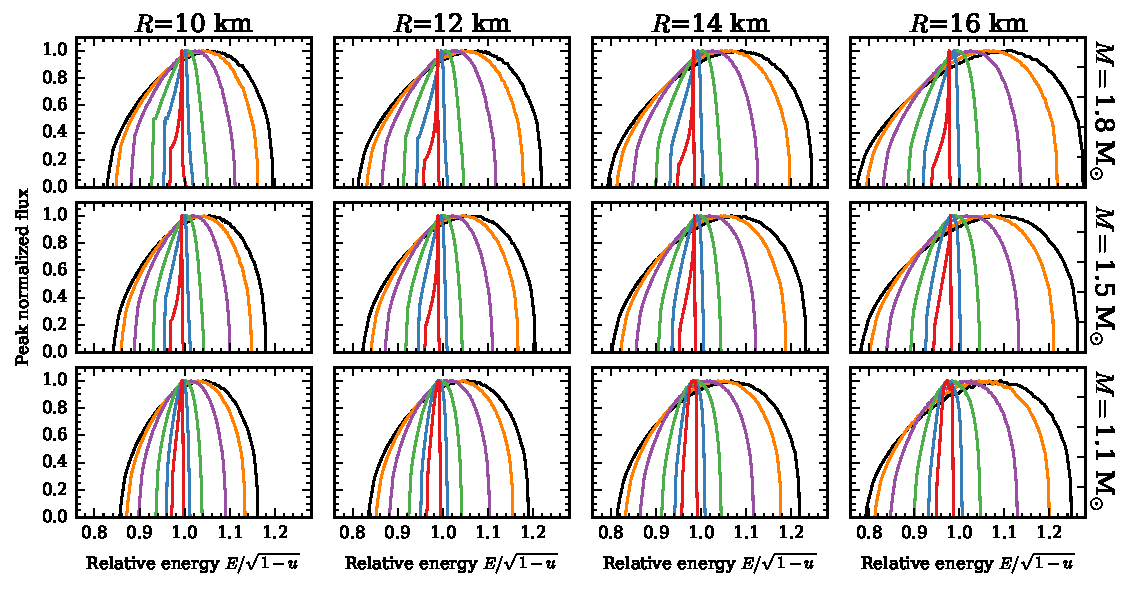
\includegraphics[width=18cm]{figs/sweep_grid.pdf}
\caption{\label{fig:sweep}
    Exact shapes of line profiles for different neutron stars spinning at $600\,\mathrm{Hz}$.
Observer inclinations span a range from $i=5\deg$ (red), $10\deg$ (blue), $20\deg$ (green), $40\deg$ (purple), $60\deg$ (orange), to $90\deg$ (black).
Energy in the horizontal axis is scaled with the compactness $\sqrt{1-u} = \sqrt{1-2GM/R_{\mathrm{e}}}$ that would be expected from the gravitational redshift alone.
Likewise, the flux in the vertical axis is always normalized with the peak flux to better show the evolution of the profile shape.
}
\end{figure*}

\begin{figure*}[htbp!]
\centering
    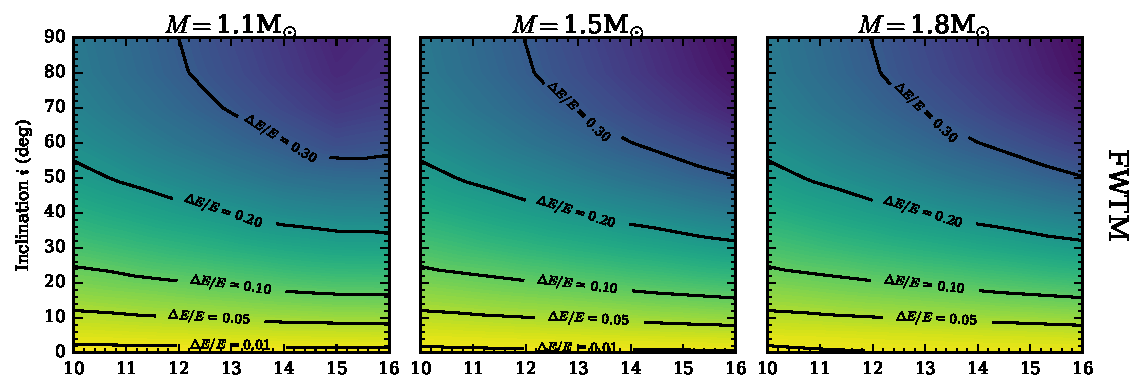
\includegraphics[width=18cm]{figs/fwhm_full.pdf}
    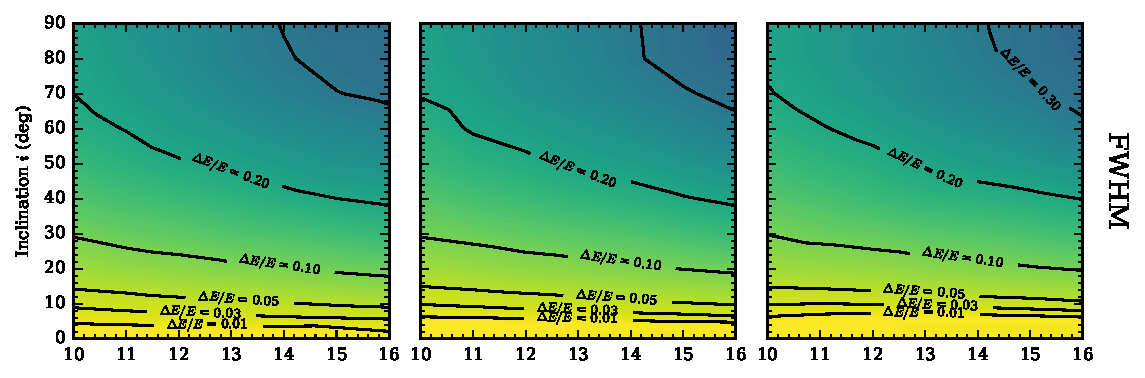
\includegraphics[width=18cm]{figs/fwhm_abs.pdf}
    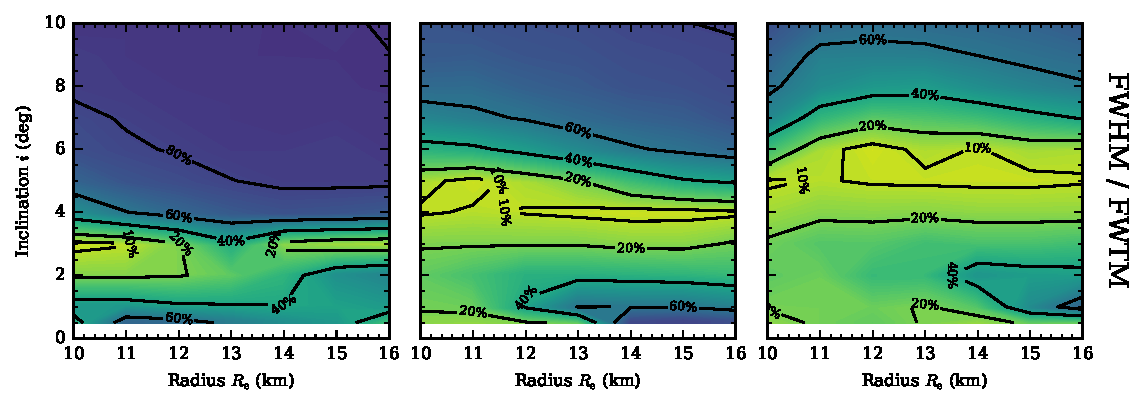
\includegraphics[width=18cm]{figs/fwhm_rel.pdf}
\caption{\label{fig:fwhm}
    Line profile Full Width at Tenth Maximum (FWTM; top row) and Full Width at Half Maximum (FWHM; middle row) as a function of radius and observer inclination computed for different neutron star configurations of $M=1.1\,\Msun$, $1.5\,\Msun$, and $1.8\,\Msun$ spinning at $600\,\mathrm{Hz}$.
    Additionally, the bottom row shows the ratio of these two that can be used to quantify how narrow the spiky part of the line profile is.
    Note the different inclination scale on the bottom row that is used to highlight the region $i < 10\deg$, where the profile evolves from a smooth to a spiky shape.
}
\end{figure*}

\refe{Next, we study the energy-dependence of the flux from the star by computing the observed energy distribution $F(E)$ of photons emitted from the stellar surface at a single energy $E'$ as measured in the comoving frame. 
\refe{In order to minimize any source of error in this section we use \textsc{arcmancer} to solve the geodesics in all of the subsequent calculations.}
Because of the variation of the redshift across the surface of the star caused by Doppler boosting and the oblate shape of the star, the observer sees a range of energies} \citep{OP03,BML06,CMB06}.
Following \citealt{Baubock15}, we are interested in constraining the convolution (smearing) kernel $\mathcal{G}(E,E')$ defined via
\be
F(E) = \int I'(E') \mathcal{G}(E,E') dE',
\ee
where we have dropped the time and angle dependency of the specific intensity $I'$ and explicitly written all quantities to be functions of the energy.
It follows from Eq. \eqref{eq:fluxint} that the actual flux of photons with an observed energy $E$ and emitted energy $E'$ is then
\begin{align}\begin{split}
    F(E) &= \iint \frac{ I'(E') }{ (1+z)^3 } \frac{bdb d\chi}{D^2} \\
         &= \iiint \frac{I'(E') }{(1+z)^4} ~ \delta \left( E - \frac{E'}{1+z} \right)  \frac{bdb d\chi}{D^2} dE',
\end{split}\end{align}
where $\delta(x)$ is the Dirac delta function.
Hence, the convolution kernel, or the so-called line profile, we are after is then 
\be
\mathcal{G}(E,E') =  \iint \frac{1}{(1+z)^4} ~\delta \left[E - \frac{E'}{1+z} \right]  \frac{bdb d\chi}{D^2}.
\ee

Examples of line profiles are shown in Fig.~\ref{fig:line_profiles} for different spacetimes and star configurations.
The flux is normalized so that the emitted bolometric flux is unity, i.e., the area encapsulated by the profile is one.
In each case, the star is taken to have $\nu = 700\,\mathrm{Hz}$, $R_{\mathrm{e}} = 10\,\mathrm{km}$, and $M=1.4\,\Msun$.
Observer inclination is $i=20^{\circ}$ and emission is taken to be isotropic, for simplicity.
\refedel{We consider a \sch spacetime for spherical and oblate stars, with radius given by Eq.~\eqref{eq:radf}, in addition to a full second-order spacetime with quadrupole moments and an oblate neutron star surface.}
\refe{
This figure shows line profiles for spherical and oblate stars, assuming for simplicity that the exterior spacetime is the Schwarzschild spacetime, as well as results for oblate stars in the appropriate second-order exterior spacetime, 
i.e., a spacetime with the appropriate quadrupole moment given by relations \eqref{eq:quad}-\eqref{eq:I}.
}

\refe{Line profiles computed using \sch metric with a spherical star appear smooth and asymmetrical with an enhancement towards higher energies caused by the relativistic Doppler boosting \citep[see e.g.][]{OP03}.}
\refe{For an oblate star the increased redshift of the regions near the pole shifts the peak towards lower energies.}
\refe{The resulting line profile is fairly symmetric \citep[see e.g.][]{BPO13}.}
\refe{However, when a physically more realistic metric with a non-zero quadrupole moment is used, the high-energy part of the line profile is further enhanced.}
\refe{This again results in an asymmetrical line profile.}
\refe{When the value of the quadrupole moment is increased to unphysically high levels the line profile develops a narrow peak in the high-energy part.}
\refe{This effect is, however, highly dependent on the observer inclination relative to the rotation axis of the star.}


Let us now study the line profile shape in full detail using the \textsc{bender} code.
In order to fully map the change in the line profile shape as a function of observer inclination, we calculated different profiles for three different cases: $M=1.1\,\Msun$, $1.5\,\Msun$, and $1.8\,\Msun$.
Here we consider only rapidly spinning stars and hence set the spin to $600\,\mathrm{Hz}$, close to the maximum value observed for AMPs.
For each mass, the equatorial radius $R_{\mathrm{e}}$ and observer inclination $i$ were taken to span the full range from $10$ to $16\,\mathrm{km}$, and $0$ to $90\deg$, respectively.
Examples of the observed line profiles are shown in Fig.~\ref{fig:sweep} for $i=5\deg$, $10\deg$, $20\deg$, $40\deg$, $60\deg$, and $90~\deg$.
From here it is easy to see that the profile appears smooth at almost all observer viewing angles.
It is only at $i \lesssim 5\deg$ that a sharp spike starts to form.
In this case, however, the actual observed width of the profile is already below $0.03 \times E$, whereas the spike is as narrow as $0.01 \times E$.
Hence, for a spectral energy feature at around $10\,\mathrm{keV}$, a resolution of $0.1\,\mathrm{keV}$ would be needed to resolve it.
\refedel{At the moment, there are no existing observational facilities with sufficient resolution to separate the compact spike from the rest of the line profile.}

We can also try and quantify the observed effect more thoroughly by introducing the Full Width at Half Maximum (FWHM) of the profile (i.e., width of the profile at $F_{\mathrm{max}}/2$).
In addition we consider the Full Width at Tenth Maximum (FWTM) that reflects the total width of the profile (i.e., width of the profile at $F_{\mathrm{max}}/10$).
These values are shown for different radii and observer inclinations in Fig.~\ref{fig:fwhm}.
They are also a useful measure of how the rotation would smear the observed spectra:
FWTM gives a quantitative estimate of how widely smeared any narrow feature, such as a line or an absorption edge, would be observed.
FWHM, on the other hand, quantifies the energy resolution needed to resolve the exact effects from rotation itself.
Finally, we can also use their ratio to describe the shape of the line profile:
more narrow (and hence localized) the line profile feature is, smaller we expect this fraction to be.
For a narrow peak we expect \refe{FWHM/FWTM} of around $\sim 10\,\%$.
This ratio is shown in the bottom panels of Fig.~\ref{fig:fwhm}.
\refe{We can see that for a star rotating at $600\,\mathrm{Hz}$, a narrow line feature is visible only for observers with inclinations in a very narrow range, i.e., $3\deg  < i < 6\deg$, irrespective of the mass or radius of the star.}


These results can be compared to the results in \citet{BPO13}. 
\refe{Here the line profiles using \sch exterior metric are seen to match well with our calculations.}
\refe{For the profiles computed using a metric which includes corrections up to second-order order in $\Ob$, we see a clear deviation.}
\refe{Most notably the line profiles we compute only contain narrow features in a very restricted range of observer inclinations $3\deg  < i < 6\deg$. }
\refe{However, \citet{BPO13} find narrow spectral features with observer inclinations $i \lesssim 30\deg$ with a similar neutron star parameters.}
\refe{A possible reason for this discrepancy can be traced back to how the value of the quadrupole moment is computed.}
\refe{The value of our quadrupole moment is derived from the scaling relations whereas \citet{BPO13} set their value of $q$ by hand.}
\refe{They use the Hartle-Thorne metric \citep{HT68} in their calculations where} the quadrupole moment is given by $\qinv = -j^2 (1 + \eta)$, where $j$ is the dimensionless spin parameter (see eq. \eqref{eq:wbar}; $a$ in the notation of \citealt{BPO13}) and $\eta$ is the strength of the deviation from a spherical potential ($\eta = 0$ reduces to Kerr-like spacetime).
\citet{BPO13} select $\eta=3.3$ that is a typical value given by the FPS EoS \citep{FPS} for a star with $M\approx1.4\,\Msun$ \citep[see][]{LP99}.
For the angular momentum they adopt $j = 0.357$, again, as given by the FPS EoS at $\nu \approx 700\,\mathrm{Hz}$.
With the aforementioned value, their quadrupole moment is then $\qinv \approx -0.548$.
Radius they imposed was $R = 10\,\mathrm{km}$.

One should, however, note that by \refe{selecting an individual EoS} and setting the \refe{star's mass and angular momentum}, the radius of the star is already determined for physically realistic parameter combinations.
In their case, the FPS EoS would yield \refe{a considerably different radius of} $R_{\mathrm{e}} \approx 11.8\,\mathrm{km}$ \citep{CST94, LP99}.
%, \refedel{an eccentricity of $\epsilon \approx 0.444$,} $\beta \approx 0.013$ \citet{CST94}, and $q \approx -0.613$ \citet{LP99}. 
%\refe{The resulting coordinate-invariant quadrupole moment is then $\qinv \approx -0.595$.}
Also it should be noted that \citet{BPO13} do not include a contribution from the pressure quadrupole moment $\beta$ into their coordinate-invariant quadrupole expression \citep{PA12}.
\refe{We, on the other hand, get for} $M=1.4\,\Msun$, $R_{\mathrm{e}}=10\,\mathrm{km}$, and $\nu = 700\,\mathrm{Hz}$ the following values: 
$j \approx 0.275$, $q \approx -0.268$, and $\beta \approx 0.010$ that then give $\qinv \approx -0.255$.
Hence, the value of the $\qinv$ used in \citet{BPO13} is approximately twice that of a physically realistic neutron star with $R_{\mathrm{e}} = 10\,\mathrm{km}$.

In general, the quadrupole moment is larger for a stiffer EoS, because a stiffer EoS produces a larger star and the quadrupole moment scales with the square of the radius.
For us, this scaling is taken into account by the relations \eqref{eq:quad} and \eqref{eq:beta} that are obtained by fitting a large library of EoSs \citep[see][]{BBP13, aGM14} to yield a consistent quadrupole moment at any given mass, radius, \refedel{(i.e., stiffness)} and angular velocity.%
\footnote{This scaling also hides the difference between the non-rotating and rotating radii because it is formulated using the equatorial radius $R_{\mathrm{e}}$.
Alternatively, one could always consider the corresponding $R_0$ of a non-rotating configuration for which $R_0 \le R_{\mathrm{e}}$ for any given $\Ob$.
\refe{This distinction between rotating and non-rotating radius is important as equation of state modeling for the cold dense matter inside neutron stars is typically done assuming non-rotating radii.}
}
%For a $M=1.4~\Msun$, $R_{\mathrm{e}}=10~\mathrm{km}$, and $\nu = 700~\mathrm{Hz}$ we obtain $j \approx 0.275$, $q \approx -0.268$, and $\beta \approx 0.010$ that then give $\qinv \approx -0.255$.
Hence, in this particular comparison, our $j$ and $\qinv$ are smaller because we demand that radius should be $10\,\mathrm{km}$.
%Additionally, a star like this with $\Ob \approx 0.323$ has an eccentricity $\epsilon \approx 0.341$ as given by the radius function \eqref{eq:radf}.
Line profile emerging from a such a star is shown with a red solid line in Fig.~\ref{fig:line_profiles} and is not seen to develop a narrow core. 
\refedel{This is because the quadrupole moment is not strong enough to dominate the countering effect of the region of increased redshift around the pole.}
%By artificially increasing the quadrupole moment to be $q \times 2$, roughly consistent with the value used in \citet{BPO13}, we do reproduce the narrow feature in the blue part of the line profile for a spherical star.
For an oblate star, we need to artificially increase $q$ by a factor of $4$, so that $q = -1.07$, in order for the line profile to produce a narrow core as seen in the red dashed line in Fig.~\ref{fig:line_profiles}.
%Here the large difference to the spherical configuration is explained by the increasing eccentricity of the star that acts as a countering \refe{effect} because it strengthens the gravitational part of the $g_{tt}$ component due to the star being more compressed, and hence more compact, around the poles.
%Hence, it is crucial to consider not only correct quadrupole moment strength but also a correct eccentricity at the same time.
In conclusion, we are only able to reproduce the narrow peak with a large observer inclination of $20\deg$, shown in fig. 2 of \citet{BPO13}, by \refe{artificially increasing the value of $q$}. 
%quadrupole moment but not with a quadrupole moment value originating from our \refedel{$q$} parameterization.

\refe{
Later on, \citet{BBP13} revised their calculations and re-computed their observed line profile in Hartle-Thorne metric with values of quadrupole moment $q$ originating from a similar physically consistent empirical parameterization.
In this case, \citet{BBP13} still find a narrow spectral feature in the line profile for a neutron star with $R_{\mathrm{e}} = 10\,\mathrm{km}$, $M=1.4\,\Msun$, and $\nu = 700\,\mathrm{Hz}$, similar to the parameters used in \citet{BPO13} (see fig. 5 \citealt{BBP13}).
However, the observer inclination was not specified.
Based on our results presented in Figures \ref{fig:sweep} and \ref{fig:fwhm} we can, however, say that the formation of a narrow peak for these neutron star parameters is only possible in a very limited range of observer inclinations around $i \sim 5\deg$.
}

%In this case, \textbf{a similar suppression of the narrow peak formation can be seen: 
%this can be inferred from the smaller width of the profile that a considerably smaller inclination is needed to create a line profile with a spiky shape (see fig. 5 in \citealt{BBP13}).}



\subsection{AMP pulse profiles}\label{sect:AMPs}

From here on, we move to time-dependent ray tracing problems by considering pulse profiles from AMPs.
Here a hot spot \refedel{on top of} \refe{on the stellar} surface is emitting and the star is seen to rotate with a frequency of $\Omega$.
\refe{The internal accuracy of the calculations is only set by the error tolerance of the numerical integration of the flux.
Hereafter we use a relative tolerance of $5 \times 10^{-3}$.
Results here were obtained using both the split Hamilton-Jacobi propagator and \textsc{arcmancer} and were seen to match perfectly given the numerical error tolerance.
For simplicity, in the following discussion we will only show the results obtained by the split Hamilton-Jacobi method.
}

\refe{
We compared our calculations to the results obtained with the forward-in-time method \citep[see e.g.,][]{PB06, MLCB07}.
Results presented here using this formulation are computed by T. Salmi and J. Poutanen (private communications) with a code described in \citet{PB06}; Salmi et al. 2018 (in preparation).
Note that here the definition of the differential surface element is given by Eq. \eqref{eq:dS_subs} and hence correctly includes the $\lgamma$ factor.
Such a comparison is crucial in order to verify that all of the physics is correctly incorporated to the formulations of the given methods.
Hence, results between the two methods should agree up to the numerical tolerance.
}

First, a general comparison of the ray tracing algorithm with the S+D approximation was done. 
For simplicity, only spherical stars were considered here.
Main parameters were: the stellar mass $M = 1.6\,\Msun$, the stellar radius $R = 12\,\mathrm{km}$, the observer inclination $i = 60^{\circ}$ and the colatitude of the spot $\theta_{\mathrm{s}} = 50^{\circ}$.  
The effective temperature of the radiation was set to $T_{\mathrm{eff}} = 2\,\mathrm{keV}$.  
The distance to the source was assumed to be $D = 10\,\mathrm{kpc}$.  
We defined a circular spot with an angular radius $\rho$ of either $1$ or $30$ degrees.
Here the spot size is defined using its angular size \refe{in the co-rotating coordinate system.}
\refedel{Hence, the spot size is measured using the \textit{angular} size, not the \textit{spatial} size.}
Angular distribution of radiation corresponds either to isotropic blackbody with constant intensity or an electron scattering dominated atmosphere, i.e., the Hopf profile.


The light curves are computed in 128 time bins.  Zero time $t = 0$ corresponds to the moment when the spot center crosses the plane defined by the spin axis and the direction to the observer.  
We computed curves for the five following quantities: monochromatic photon flux ($\mathrm{ph}\,\mathrm{cm}^{-2}\,\mathrm{s}^{-1}\,\mathrm{keV}^{-1}$) at the observer energies $E = 2,~6$ and $12\,\mathrm{keV}$, bolometric photon flux ($\mathrm{ph}\,\mathrm{cm}^{-2}\,\mathrm{s}^{-1}$), and the bolometric energy flux ($\mathrm{erg}\,\mathrm{cm}^{-2}\,\mathrm{s}^{-1}$).


\begin{figure*}
\centering
\includegraphics[width=18cm]{figs/fig2a.pdf}
\caption{\label{fig:sch_comp1}
  Light curve comparisons for \sch spacetime with slowly rotating spherical star ($R = 12\,\mathrm{km}$, $M = 1.6\,\Msun$, $\nu = 1\,\mathrm{Hz}$, $i = 60^{\circ}$, $\theta_{\mathrm{s}} = 50^{\circ}$, $\rho = 1^{\circ}$, and $T_{\mathrm{eff}} = 2\,\mathrm{keV}$) emitting according to blackbody or Hopf profile with spot size either $1$ or $30$ degrees.
    Black solid line shows the pulse profiles computed using the S+D approximation \refe{(forward-in-time method; see text)} and red dashed line is a profile computed with the code presented here.
  The lower panel shows the residuals as $\Delta = (\mathrm{model_{S+D}}/\mathrm{model} -1) \times 100\%$.
}
\end{figure*}

\begin{figure*}
\centering
\includegraphics[width=18cm]{figs/fig2b.pdf}
\caption{\label{fig:sch_comp400}
  Light curve comparisons for \sch spacetime with rapidly rotating spherical star ($\nu = 400\,\mathrm{Hz}$).
  Otherwise the parameters and symbols are the same is in Fig.~\ref{fig:sch_comp1}.
}
\end{figure*}


Comparison of these lightcurves are shown in Fig.~\ref{fig:sch_comp1} for slowly rotating star ($1$ Hz) and in Fig.~\ref{fig:sch_comp400} for fast rotation ($400$ Hz).
In practice, comparing the profiles for slow rotation only tests our ray tracing routines because special relativistic effects (Doppler boosting, angle aberration and so on) are negligible.
Overall agreement of the two different methods is excellent and from here a baseline accuracy of about $<0.2\%$ relative error is obtained for the mapping of quantities between image plane and star's surface.
No large deviation between isotropic and Hopf profile is detected either, indicating a good agreement in our emission angle computations and formulation.
Similarly, when rotation is increased and special relativistic effects start to play a role we are able to reproduce the pulse profiles usually down to $<0.3\%$ relative error, except near $\phi_{\mathrm{e}} \sim 0$.
Here the tilt of the spot increases and even though the absolute error remains the same, the relative error grows because the observed flux is smaller and smaller for a more inclined spot.
Such a situation is numerically expensive to deal when integrating the observed flux from the NS image.
In this case, we set set a bound on the number of flux integrand evaluations (typically $\sim 10^7$ function calls) that in effect set an absolute error for the flux.
It is then only in these rare cases that our integrator does not respect the relative error criteria set by us.

%\subsection{Oblate Schwarzchild $+$ Doppler}

%\begin{figure*}
%\centering
%\includegraphics[width=16cm]{figs/fig3.pdf}
%\caption{\label{fig:sch_obl}
%  Bolometric energy flux comparisons for oblate Schwarzchild approximation with rapidly rotating star ($R_{\mathrm{eq}} = 16.4~\mathrm{km}$, $M = 1.4~\Msun$, $\nu = 600~\mathrm{Hz}$, and $\rho = 1^{\circ}$).
%  Left panel shows a pulse profile as compared to fig. 3 in \cite{MLCB07} with $i = 70^{\circ}$ and $\theta_s = 49^{\circ}$.
%  The spherical star is taken to have $R(49^{\circ}) = 15.1~\mathrm{km}$.
%  Right panel can be compared against fig. 4 in \cite{MLCB07} with $i = 20^{\circ}$ and $\theta_s = 41^{\circ}$
%  In this case, the spherical star has $R(41^{\circ}) = 14.8~\mathrm{km}$.
%}
%\end{figure*}


\begin{figure*}
\centering
\includegraphics[width=18cm]{figs/fig4.pdf}
\caption{\label{fig:osch_comp700}
  Light curve comparisons for oblate \sch spacetimes with three different spot colatitudes: $\theta_{\mathrm{s}} = 18^{\circ}$, $45^{\circ}$ and $90^{\circ}$.
  Additionally, the bottom row shows comparison of pulse profile for electron scattering atmosphere for $\theta_{\mathrm{s}} = 45^{\circ}$.
  Parameters of the star, spot and observer are: $R_{\mathrm{e}} = 12.0\,\mathrm{km}$, $M = 1.4\,\Msun$, $\nu = 700\,\mathrm{Hz}$, $i = 45^{\circ}$ and $\rho = 10^{\circ}$.
  Otherwise the parameters and symbols are the same is in Fig.~\ref{fig:sch_comp1}.
  }
\end{figure*}

Next we compare emission from oblate stars.
The surface here is defined using the radius function \eqref{eq:radf} but the star is still embedded in a symmetric \sch spacetime.
The parameters used are equatorial radius $R_{\mathrm{e}} = 12\,\mathrm{km}$ (in the usual \sch metric), neutron star mass of $M = 1.4\,\Msun$, extreme rotational frequency $\nu = 700\,\mathrm{Hz}$, observer inclination $i=45^{\circ}$, and spot angular size of $\rho = 10^{\circ}$.
Effective temperature of the radiation is again taken to be $T_{\mathrm{eff}} = 2\,\mathrm{keV}$, and the distance to be $D = 10\,\mathrm{kpc}$.
Here the spot size is defined in a \refe{co-rotating} spherical coordinate system on top of a unit sphere and is then projected to the oblate inclined surface.
To trace the effects of the changing surface we consider the spot in three different locations at colatitudes of $\theta_{\mathrm{s}} = 18^{\circ}$, $45^{\circ}$, and $90^{\circ}$.
Additionally, we consider a spot with angle-dependent emission intensity.
This is done using the electron scattering atmosphere with $\theta_{\mathrm{s}} = 45^{\circ}$.
%Additionally for $\theta_{\mathrm{s}} = 90^{\circ}$ when the spot is on the equator we observer a full eclipse in the light curve.
%This imposes a serious test for both of the codes as the gradually more and more blocked spot is also seen from a very shallow angle before disappearing and appearing again.
%We note that when integrating flux from the spot in the image plane, a polar subgrid is extremely useful just before the eclipse as the impact parameter can vary only by a $\sim1\%$ before the spot is hidden behind the star.
%Attaining a similar resolution in a Cartesian subgrid would then need far more integrand evaluations as the spot is seen from a very shallow angle.

A comparison of the oblate lightcurves is shown in Fig.~\ref{fig:osch_comp700}.
Again we obtain an excellent agreement with the forward-in-time method, with similar errors as in the spherical case (relative error $< 0.2\%$).
This agreement is, of course, expected since our method is general and does not depend on the shape of the emitting surface.
The only large deviation is again seen when the spot is viewed from an extreme angle for $\theta_{\mathrm{s}} = 90^{\circ}$, just before the \refedel{eclipse}\refe{occultation}.
\refe{Hence, conclude that the two methods, forward-in-time and backwards-in-time, agree all the way up to the numerical tolerance.}

%\subsection{Hartle-Thorne -like spacetimes}
%\begin{figure*}
%\centering
%\includegraphics[width=18cm]{figs/fig5.pdf}
%\caption{\label{fig:sch_comp400}
%  Light curve comparisons for Hartle-Thorne spacetime with rapidly rotating oblate stars.
%}
%\end{figure*}


\begin{figure*}
%\centering
\includegraphics[width=18cm, height=20cm]{figs/fig7.pdf}
\caption{\label{fig:skymap}
    Skymaps of the emitted radiation as produces by rapidly rotating, oblate AMP with one or two antipodal spots.
    Star is taken to have $R_{\mathrm{e}} = 15\,\mathrm{km}$, $M=1.6\,\Msun$, and $\nu = 600\,\mathrm{Hz}$.
    Spot sizes are $\rho = 10^{\circ}$ and the emission is coming from an isotropic black body with $T_{\mathrm{eff}} = 2\,\mathrm{keV}$.
    Red curves enclose the area where \refedel{eclipses}\refe{occultation} are observed.
  }
\end{figure*}

\begin{figure}
%\centering
\includegraphics[width=8.5cm]{figs/fig8.pdf}
\caption{\label{fig:pulsefracs}
    Pulse fractions observed from rapidly rotating oblate AMP.
    Parameters of the star and the spot(s) are the same as in Fig.~\ref{fig:skymap}.
  }
\end{figure}


As a last example, after the comparisons, we calculate full skymaps of the emerging radiation from rapidly rotating oblate AMPs as shown in Fig.~\ref{fig:skymap}.
The emission from the AMP is shown for all possible observers and is mapped to the vertical axis by using the observer's inclination angle $i$.
Horizontal axis of the map is the usual pulse phase.
The brightness of the skymap is proportional to the received bolometric photon number flux.
Taking a slice of the skymap at one particular value of $i$ produces the light curve as seen by the observer at that inclination.
Calculations here are done for an extreme case of a NS with $R_{\mathrm{e}} = 15\,\mathrm{km}$, $M=1.6\,\Msun$, and $\nu = 600\,\mathrm{Hz}$.
Spot size of $\rho = 10^{\circ}$ is considered, with varying co-latitudes ranging from near the pole at $\theta_{\mathrm{s}} = 10^{\circ}$ to the equator at $\theta_{\mathrm{s}} = 90^{\circ}$.
We consider both the cases of one spot and two antipodal spots with isotropic beaming and black body emission with $T_{\mathrm{eff}} = 2\,\mathrm{keV}$.
As a result, we can see that full \refe{occultations} are only observed with one spot.
From here it is also easy to see how the maxima and minima of the flux varies in phase when the viewing angle of the observer is changing.
The effect becomes the most prominent with two spots located at $\theta_{\mathrm{s}} \sim 50-70^{\circ}$ (second antipodal spot at $\theta_{\mathrm{s,2}} \sim 110-130^{\circ}$) and the minimum is seen to change from around phase 0.2 all the way to 0.4.

We also show the corresponding strength of the observed pulsations for each inclination and spot co-latitude combinations in Fig.~\ref{fig:pulsefracs}.
Here the color of the image corresponds to the pulse fraction computed by
\be
f_p = \frac{F_{\mathrm{max}} - F_{\mathrm{min}}}{F_{\mathrm{max}} + F_{\mathrm{min}}},
\ee
where $F_{\mathrm{min}}$ and $F_{\mathrm{max}}$ are the minimum and maximum values in the bolometric light curves, respectively.
From here the symmetry between $\theta_{\mathrm{s}}$ and $i$ becomes obvious as the lines of constant amplitude appear almost symmetric against switching between $x$ and $y$ axis.




\section{Summary}\label{sect:summary}
We have presented a detailed study of radiation emerging from and near rotating compact objects.
A framework of formulae for solving this problem was derived in a fully general relativistic manner. 
The formulae were then specialized to the context of rotating neutron stars.


Firstly, in Section \ref{sect:spacetime} we gave a detailed description of the second-order in rotation spacetime metric that was used.
The spacetime we use has a non-zero coordinate-invariant mass quadrupole moment $\qinv$. 
\refe{The components $q$ and $\beta$ of $\qinv$ are defined via approximate relations for a wide span of neutron star masses, radii, and spins, following \citet{aGM14}.}
When the rotation increases, the star also starts to deviate from a sphere due to the weakening of the gravitational force on the equator because of the increasing centrifugal force.
An \refe{approximate} relation for the resulting oblate spheroidal shape of the star can, however, again be obtained \citep{MLC07, aGM14} and was implemented in Section \ref{sect:oblate} for an easy but consistent description of the surface.

Secondly, we derived a new, \refe{approximate} ray-tracing \refe{approach} using the so-called split Hamilton-Jacobi (also known as super-Hamiltonian) method.
This derivation is presented and discussed in detail in Sections \ref{sect:hamjac} and \ref{sect:raytracing}.
Instead of using the geodesic equation that is a second-order differential equation we separate the Hamilton-Jacobi equation using a third constant of motion known as Carter's constant.
The method is exact up to first-order in rotation (Kerr-like spacetime with frame-dragging effects) but remains sufficiently accurate also for second order in rotation because deviations caused by the quadrupole moments are small.
Formulating the components of the four-momentum vector like this has the useful feature that the polarization of the radiation can easily be taken into account \citep[see e.g.][]{cha, dexter2016}

Thirdly, we gave a thorough description of the calculations related to the actual emission of the radiation.
Effects like redshift, Doppler boosting and emission angle of the photon were discussed in a fully general relativistic manner in Sections \ref{sect:redshift_angle} and \ref{sect:emission}. 
\refedel{,hence also verifying the previous ad-hoc special relativistic formulations}% \citep[see e.g.][]{PG03, PB06}.}
In the special relativistic formulation \citep[see e.g.,][]{PB06} the calculations are done in a flat spacetime and then Lorentz boosted to the rotating relativistic frame.
%In Section \ref{sect:coords}, we \refedel{derived a connection to}\refe{expand} this method by introducing a way to measure the angular size of a pattern in the co-rotating frame.
%\refe{This result highlights how it is crucial to specify if the pattern size is defined using linear or angular sizes when dealing with rotating coordinate systems in special relativity.}
%\refe{Derivation of the} full solid angle element is also \refe{shown} that can then be used with forward-in-time \refe{formulations so that the results match with the backwards-in-time formulation, as one expects from purely physical arguments}.
%\refedel{Most notably, this leads to an addition of $\lgamma$, a Lorentz boost factor, on the observed flux, understood to originate from a simple Lorentz contraction in \sch metric.}
\refe{In Section \ref{sect:coords}, we present a derivation of the solid angle element defined using rotating coordinate system.}
\refe{The purpose of this is to clarify some common misunderstandings in the literature of how such a transformation from the co-rotating to the static coordinate system can be done.}
We also briefly discussed the actual intensity of the emerging radiation and \refe{presented} an iterative method to solve the Chandrasekhar-Ambartsumian integral, along a new approximative polynomial expansion, that is related to the angle-dependent electron scattering atmosphere, in Section \ref{sect:angular_distr}.
We then describe the actual intensity of the emerging radiation and as a simple model use the angle-dependent electron scattering atmosphere, presented in Section \ref{sect:angular_distr}.
%and review an iterative method to solve the Chandrasekhar-Ambartsumian integral, along a new approximative polynomial expansion, that is related to the angle-dependent electron scattering atmosphere, in Section \ref{sect:angular_distr}.
Numerical methods to solve all of the presented equations were then laid out in Section \ref{sect:num_methods}.

Finally, in Section \ref{sect:appl} we presented some applications of the framework.
Connection to previous work in the literature was also made, when possible.
As a first simple example, we showed how the image of NS is formed in a curved spacetime.
Next, we studied the energy dependent emission by considering the emerging line profiles.
Most notably, we concluded that when a consistent formulation is used for how the increasing eccentricity of the star is coupled with the related quadrupole moments, no narrow features are seen in the line profiles.
We then did an extensive and thorough study of AMP pulse profiles and compared our results to results obtained using existing special relativistic methods found in the literature.
Here the agreement between the two methods was found to be excellent \refe{when the correct differential surface area element presented in Sect. \ref{sect:coords} is used}.
Lastly, we computed full skymaps of radiation emerging from rapidly rotating AMPs, taking into account the oblate shape of the star and the quadrupole moments of the spacetime metric.



%\section{Conclusions}
\section*{Acknowledgments}

\small{
We offer sincere thanks to various people that helped to improve the formulation of the theory and the actual paper by engaging the authors to helpful discussions: 
Most notably we would like to thank Juri Poutanen, Cole Miller, Fred Lamb, \refe{Jean in't Zand}, and Sharon Morsink for their help and comments.
We also offer special thanks to Tuomo Salmi for producing us the pulse profiles for the code comparison.
JN acknowledges support from the University of Turku Graduate School in Physical and Chemical Sciences.
PP acknowledges support from the Academy of Finland, grant no.~1274931.

This work benefited from discussions at the International Symposium on Neutron Stars in the Multi-Messenger Era in May 2016 supported by the National Science Foundation under Grant No. PHY-1430152 (JINA Center for the Evolution of the Elements).
%\red{INT2b-1r pre-print number}
}


\bibliographystyle{aa}
\bibliography{allbib}

% \begin{thebibliography}{55}
% \expandafter\ifx\csname natexlab\endcsname\relax\def\natexlab#1{#1}\fi
% 
% \bibitem[{{Agrawal}(2006)}]{Astrosat}
% {Agrawal}, P.~C. 2006, Advances in Space Research, 38, 2989
% 
% \bibitem[{{AlGendy} \& {Morsink}(2014)}]{aGM14}
% {AlGendy}, M. \& {Morsink}, S.~M. 2014, \apj, 791, 78
% 
% \bibitem[{{Bardeen} \& {Wagoner}(1971)}]{BW71}
% {Bardeen}, J.~M. \& {Wagoner}, R.~V. 1971, \apj, 167, 359
% 
% \bibitem[{{Baub{\"o}ck} {et~al.}(2013{\natexlab{a}}){Baub{\"o}ck}, {Berti},
%   {Psaltis}, \& {{\"O}zel}}]{BBP13}
% {Baub{\"o}ck}, M., {Berti}, E., {Psaltis}, D., \& {{\"O}zel}, F.
%   2013{\natexlab{a}}, \apj, 777, 68
% 
% \bibitem[{{Baub{\"o}ck} {et~al.}(2015){Baub{\"o}ck}, {{\"O}zel}, {Psaltis}, \&
%   {Morsink}}]{Baubock15}
% {Baub{\"o}ck}, M., {{\"O}zel}, F., {Psaltis}, D., \& {Morsink}, S.~M. 2015,
%   \apj, 799, 22
% 
% \bibitem[{{Baub{\"o}ck} {et~al.}(2013{\natexlab{b}}){Baub{\"o}ck}, {Psaltis},
%   \& {{\"O}zel}}]{BPO13}
% {Baub{\"o}ck}, M., {Psaltis}, D., \& {{\"O}zel}, F. 2013{\natexlab{b}}, \apj,
%   766, 87
% 
% \bibitem[{{Baub{\"o}ck} {et~al.}(2012){Baub{\"o}ck}, {Psaltis}, {{\"O}zel}, \&
%   {Johannsen}}]{BPO12}
% {Baub{\"o}ck}, M., {Psaltis}, D., {{\"O}zel}, F., \& {Johannsen}, T. 2012,
%   \apj, 753, 175
% 
% \bibitem[{{Bhattacharyya} {et~al.}(2006){Bhattacharyya}, {Miller}, \&
%   {Lamb}}]{BML06}
% {Bhattacharyya}, S., {Miller}, M.~C., \& {Lamb}, F.~K. 2006, \apj, 644, 1085
% 
% \bibitem[{{Braje} {et~al.}(2000){Braje}, {Romani}, \& {Rauch}}]{BR01}
% {Braje}, T.~M., {Romani}, R.~W., \& {Rauch}, K.~P. 2000, \apj, 531, 447
% 
% \bibitem[{{Butterworth} \& {Ipser}(1976)}]{BI76}
% {Butterworth}, E.~M. \& {Ipser}, J.~R. 1976, \apj, 204, 200
% 
% \bibitem[{{Cadeau} {et~al.}(2005){Cadeau}, {Leahy}, \& {Morsink}}]{CL05}
% {Cadeau}, C., {Leahy}, D.~A., \& {Morsink}, S.~M. 2005, \apj, 618, 451
% 
% \bibitem[{{Cadeau} {et~al.}(2007){Cadeau}, {Morsink}, {Leahy}, \&
%   {Campbell}}]{CML07}
% {Cadeau}, C., {Morsink}, S.~M., {Leahy}, D., \& {Campbell}, S.~S. 2007, \apj,
%   654, 458
% 
% \bibitem[{{Chan} {et~al.}(2013){Chan}, {Psaltis}, \& {{\"O}zel}}]{CPO13}
% {Chan}, C.-k., {Psaltis}, D., \& {{\"O}zel}, F. 2013, \apj, 777, 13
% 
% \bibitem[{{Chandrasekhar}(1960)}]{Cha60}
% {Chandrasekhar}, S. 1960, {Radiative transfer} (Dover, New York)
% 
% \bibitem[{Chandrasekhar(1998)}]{cha}
% Chandrasekhar, S. 1998, The Mathematical Theory of Black Holes, The International series of monographs on physics (Oxford Univ. Press, Oxford)
% 
% \bibitem[{{Chang} {et~al.}(2006){Chang}, {Morsink}, {Bildsten}, \&
%   {Wasserman}}]{CMB06}
% {Chang}, P., {Morsink}, S., {Bildsten}, L., \& {Wasserman}, I. 2006, \apjl,
%   636, L117
% 
% \bibitem[{{Cook} {et~al.}(1994){Cook}, {Shapiro}, \& {Teukolsky}}]{CST94}
% {Cook}, G.~B., {Shapiro}, S.~L., \& {Teukolsky}, S.~A. 1994, \apj, 424, 823
% 
% \bibitem[{{Dexter}(2016)}]{dexter2016}
% {Dexter}, J. 2016, \mnras, 462, 115
% 
% \bibitem[{{Dexter} \& {Agol}(2009)}]{dexter2009}
% {Dexter}, J. \& {Agol}, E. 2009, \apj, 696, 1616
% 
% \bibitem[{Friedman \& Stergioulas(2013)}]{rcs}
% Friedman, J. \& Stergioulas, N. 2013, Rotating Relativistic Stars, Cambridge
%   Monographs on Mathematical Physics (Cambridge University Press, Cambridge)
% 
% \bibitem[{{Friedman} {et~al.}(1986){Friedman}, {Ipser}, \& {Parker}}]{FIP86}
% {Friedman}, J.~L., {Ipser}, J.~R., \& {Parker}, L. 1986, \apj, 304, 115
% 
% \bibitem[{{Gendreau} {et~al.}(2012){Gendreau}, {Arzoumanian}, \&
%   {Okajima}}]{NICER}
% {Gendreau}, K.~C., {Arzoumanian}, Z., \& {Okajima}, T. 2012, in \procspie, Vol.
%   8443, Space Telescopes and Instrumentation 2012: Ultraviolet to Gamma Ray,
%   844313
% 
% \bibitem[{{Hartle} \& {Thorne}(1968)}]{HT68}
% {Hartle}, J.~B. \& {Thorne}, K.~S. 1968, \apj, 153, 807
% 
% \bibitem[{{Laarakkers} \& {Poisson}(1999)}]{LP99}
% {Laarakkers}, W.~G. \& {Poisson}, E. 1999, \apj, 512, 282
% 
% \bibitem[{{Lind} \& {Blandford}(1985)}]{LB85}
% {Lind}, K.~R. \& {Blandford}, R.~D. 1985, \apj, 295, 358
% 
% \bibitem[{{Lo} {et~al.}(2013){Lo}, {Miller}, {Bhattacharyya}, \&
%   {Lamb}}]{LMB13}
% {Lo}, K.~H., {Miller}, M.~C., {Bhattacharyya}, S., \& {Lamb}, F.~K. 2013, \apj,
%   776, 19
% 
% \bibitem[{{Lorenz} {et~al.}(1993){Lorenz}, {Ravenhall}, \& {Pethick}}]{FPS}
% {Lorenz}, C.~P., {Ravenhall}, D.~G., \& {Pethick}, C.~J. 1993, Physical Review
%   Letters, 70, 379
% 
% \bibitem[{{Misner} {et~al.}(1973){Misner}, {Thorne}, \& {Wheeler}}]{MTW73}
% {Misner}, C.~W., {Thorne}, K.~S., \& {Wheeler}, J.~A. 1973, Gravitation, (W.H.~Freeman and Co., San Francisco)
% 
% \bibitem[{{Morsink} {et~al.}(2007){Morsink}, {Leahy}, {Cadeau}, \&
%   {Braga}}]{MLC07}
% {Morsink}, S.~M., {Leahy}, D.~A., {Cadeau}, C., \& {Braga}, J. 2007, \apj, 663,
%   1244
% 
% \bibitem[{{Muno} {et~al.}(2002){Muno}, {Chakrabarty}, {Galloway}, \&
%   {Psaltis}}]{MC02}
% {Muno}, M.~P., {Chakrabarty}, D., {Galloway}, D.~K., \& {Psaltis}, D. 2002,
%   \apj, 580, 1048
% 
% \bibitem[{{Narayan} {et~al.}(2016){Narayan}, {Zhu}, {Psaltis}, \& {Sa{\c
%   d}owski}}]{NZP16}
% {Narayan}, R., {Zhu}, Y., {Psaltis}, D., \& {Sa{\c d}owski}, A. 2016, \mnras,
%   457, 608
% 
% \bibitem[{{{\"O}zel} \& {Psaltis}(2003)}]{OP03}
% {{\"O}zel}, F. \& {Psaltis}, D. 2003, \apjl, 582, L31
% 
% \bibitem[{{Page}(1995)}]{P95}
% {Page}, D. 1995, \apj, 442, 273
% 
% \bibitem[{{Papitto} {et~al.}(2014){Papitto}, {Torres}, {Rea}, \&
%   {Tauris}}]{PTR14}
% {Papitto}, A., {Torres}, D.~F., {Rea}, N., \& {Tauris}, T.~M. 2014, \aap, 566,
%   A64
% 
% \bibitem[{{Pappas} \& {Apostolatos}(2012)}]{PA12}
% {Pappas}, G. \& {Apostolatos}, T.~A. 2012, Physical Review Letters, 108, 231104
% 
% \bibitem[{{Patruno} \& {Watts}(2012)}]{PW12}
% {Patruno}, A. \& {Watts}, A.~L. 2012, ArXiv e-prints \eprint{[arXiv:1206.2727]}
% 
% \bibitem[{{Pechenick} {et~al.}(1983){Pechenick}, {Ftaclas}, \& {Cohen}}]{PFC83}
% {Pechenick}, K.~R., {Ftaclas}, C., \& {Cohen}, J.~M. 1983, \apj, 274, 846
% 
% \bibitem[{{Pihajoki} {et~al.}(2016){Pihajoki}, {Rantala}, \&
%   {Johansson}}]{PRJ16}
% {Pihajoki}, P., {Rantala}, A., \& {Johansson}, P.~H. 2016, ArXiv e-prints \eprint{[arXiv:1612.02828]}
% 
% \bibitem[{{Poutanen} \& {Beloborodov}(2006)}]{PB06}
% {Poutanen}, J. \& {Beloborodov}, A.~M. 2006, \mnras, 373, 836
% 
% \bibitem[{{Poutanen} \& {Gierli{\'n}ski}(2003)}]{PG03}
% {Poutanen}, J. \& {Gierli{\'n}ski}, M. 2003, \mnras, 343, 1301
% 
% \bibitem[{{Psaltis} \& {Johannsen}(2012)}]{PJ12}
% {Psaltis}, D. \& {Johannsen}, T. 2012, \apj, 745, 1
% 
% \bibitem[{{Psaltis} \& {{\"O}zel}(2014)}]{PO14}
% {Psaltis}, D. \& {{\"O}zel}, F. 2014, \apj, 792, 87
% 
% \bibitem[{{Pu} {et~al.}(2016){Pu}, {Yun}, {Younsi}, \& {Yoon}}]{PYY16}
% {Pu}, H.-Y., {Yun}, K., {Younsi}, Z., \& {Yoon}, S.-J. 2016, \apj, 820, 105
% 
% \bibitem[{{Rybicki} \& {Lightman}(1979)}]{RL79}
% {Rybicki}, G.~B. \& {Lightman}, A.~P. 1979, {Radiative processes in
%   astrophysics} (Wiley-Interscience, New York)
% 
% \bibitem[{{Schnittman} \& {Krolik}(2013)}]{SK13}
% {Schnittman}, J.~D. \& {Krolik}, J.~H. 2013, \apj, 777, 11
% 
% \bibitem[{{Shcherbakov} \& {McKinney}(2013)}]{SM13}
% {Shcherbakov}, R.~V. \& {McKinney}, J.~C. 2013, \apjl, 774, L22
% 
% \bibitem[{{Sobolev}(1963)}]{Sob63}
% {Sobolev}, V.~V. 1963, {A treatise on radiative transfer} (Van Nostrand, Princeton)
% 
% \bibitem[{{Soffitta} {et~al.}(2013){Soffitta}, {Barcons}, {Bellazzini},
%   {Braga}, {Costa}, {Fraser}, {Gburek}, {Huovelin}, {Matt}, {Pearce},
%   {Poutanen}, {Reglero}, {Santangelo}, {Sunyaev}, {Tagliaferri}, {Weisskopf},
%   {Aloisio}, {Amato}, {Attin{\'a}}, {Axelsson}, {Baldini}, {Basso}, {Bianchi},
%   {Blasi}, {Bregeon}, {Brez}, {Bucciantini}, {Burderi}, {Burwitz}, {Casella},
%   {Churazov}, {Civitani}, {Covino}, {Curado da Silva}, {Cusumano}, {Dadina},
%   {D'Amico}, {De Rosa}, {Di Cosimo}, {Di Persio}, {Di Salvo}, {Dovciak},
%   {Elsner}, {Eyles}, {Fabian}, {Fabiani}, {Feng}, {Giarrusso}, {Goosmann},
%   {Grandi}, {Grosso}, {Israel}, {Jackson}, {Kaaret}, {Karas}, {Kuss}, {Lai},
%   {Rosa}, {Larsson}, {Larsson}, {Latronico}, {Maggio}, {Maia}, {Marin},
%   {Massai}, {Mineo}, {Minuti}, {Moretti}, {Muleri}, {O'Dell}, {Pareschi},
%   {Peres}, {Pesce}, {Petrucci}, {Pinchera}, {Porquet}, {Ramsey}, {Rea},
%   {Reale}, {Rodrigo}, {R{\'o}{\.z}a{\'n}ska}, {Rubini}, {Rudawy}, {Ryde},
%   {Salvati}, {de Santiago}, {Sazonov}, {Sgr{\'o}}, {Silver}, {Spandre},
%   {Spiga}, {Stella}, {Tamagawa}, {Tamborra}, {Tavecchio}, {Teixeira Dias}, {van
%   Adelsberg}, {Wu}, \& {Zane}}]{XIPE}
% {Soffitta}, P., {Barcons}, X., {Bellazzini}, R., {et~al.} 2013, Experimental
%   Astronomy, 36, 523
% 
% \bibitem[{{Terrell}(1959)}]{Terrell60}
% {Terrell}, J. 1959, Physical Review, 116, 1041
% 
% \bibitem[{{Vincent} {et~al.}(2011){Vincent}, {Paumard}, {Gourgoulhon}, \&
%   {Perrin}}]{Vincent11}
% {Vincent}, F.~H., {Paumard}, T., {Gourgoulhon}, E., \& {Perrin}, G. 2011,
%   Classical and Quantum Gravity, 28, 225011
% 
% \bibitem[{{Watts}(2012)}]{Watts12}
% {Watts}, A.~L. 2012, \araa, 50, 609
% 
% \bibitem[{{Weinberg} {et~al.}(2001){Weinberg}, {Miller}, \& {Lamb}}]{WM01}
% {Weinberg}, N., {Miller}, M.~C., \& {Lamb}, D.~Q. 2001, \apj, 546, 1098
% 
% \bibitem[{{Wijnands} \& {van der Klis}(1998)}]{WvdK98}
% {Wijnands}, R. \& {van der Klis}, M. 1998, \nat, 394, 344
% 
% \bibitem[{{Yagi} \& {Yunes}(2013)}]{YY13}
% {Yagi}, K. \& {Yunes}, N. 2013, Science, 341, 365
% 
% \bibitem[{{Zhang} {et~al.}(2016){Zhang}, {Feroci}, {Santangelo}, {Dong},
%   {Feng}, {Lu}, {Nandra}, {Wang}, {Zhang}, {Bozzo}, {Brandt}, {De Rosa}, {Gou},
%   {Hernanz}, {van der Klis}, {Li}, {Liu}, {Orleanski}, {Pareschi}, {Pohl},
%   {Poutanen}, {Qu}, {Schanne}, {Stella}, {Uttley}, {Watts}, {Xu}, {Yu}, {in 't
%   Zand}, {Zane}, {Alvarez}, {Amati}, {Baldini}, {Bambi}, {Basso},
%   {Bhattacharyya}, {Bellazzini}, {Belloni}, {Bellutti}, {Bianchi}, {Brez},
%   {Bursa}, {Burwitz}, {Budtz-Jorgensen}, {Caiazzo}, {Campana}, {Cao},
%   {Casella}, {Chen}, {Chen}, {Chen}, {Chen}, {Chen}, {Chen}, {Civitani}, {Coti
%   Zelati}, {Cui}, {Cui}, {Dai}, {Del Monte}, {De Martino}, {Di Cosimo},
%   {Diebold}, {Dovciak}, {Donnarumma}, {Doroshenko}, {Esposito}, {Evangelista},
%   {Favre}, {Friedrich}, {Fuschino}, {Galvez}, {Gao}, {Ge}, {Gevin}, {Goetz},
%   {Han}, {Heyl}, {Horak}, {Hu}, {Huang}, {Huang}, {Hudec}, {Huppenkothen},
%   {Israel}, {Ingram}, {Karas}, {Karelin}, {Jenke}, {Ji}, {Kennedy}, {Korpela},
%   {Kunneriath}, {Labanti}, {Li}, {Li}, {Li}, {Liang}, {Limousin}, {Lin},
%   {Ling}, {Liu}, {Liu}, {Liu}, {Lu}, {Lund}, {Lai}, {Luo}, {Luo}, {Ma},
%   {Mahmoodifar}, {Marisaldi}, {Martindale}, {Meidinger}, {Men}, {Michalska},
%   {Mignani}, {Minuti}, {Motta}, {Muleri}, {Neilsen}, {Orlandini}, {Pan},
%   {Patruno}, {Perinati}, {Picciotto}, {Piemonte}, {Pinchera}, {Rachevski},
%   {Rapisarda}, {Rea}, {Rossi}, {Rubini}, {Sala}, {Shu}, {Sgro}, {Shen},
%   {Soffitta}, {Song}, {Spandre}, {Stratta}, {Strohmayer}, {Sun}, {Svoboda},
%   {Tagliaferri}, {Tenzer}, {Tong}, {Taverna}, {Torok}, {Turolla}, {Vacchi},
%   {Wang}, {Wang}, {Walton}, {Wang}, {Wang}, {Wang}, {Wang}, {Weng}, {Wilms},
%   {Winter}, {Wu}, {Wu}, {Xiong}, {Xu}, {Xue}, {Yan}, {Yang}, {Yang}, {Yang},
%   {Yuan}, {Yuan}, {Yuan}, {Zampa}, {Zampa}, {Zdziarski}, {Zhang}, {Zhang},
%   {Zhang}, {Zhang}, {Zhang}, {Zhang}, {Zheng}, {Zhou}, \& {Zhou}}]{eXTP}
%   {Zhang}, S.~N., {Feroci}, M., {Santangelo}, A., {et~al.} 2016, ArXiv e-prints \eprint{[arXiv:1607.08823]}
% 
% \end{thebibliography}




\end{document}
